\documentclass[a4paper,10pt]{article}
\usepackage[utf8]{inputenc}
\usepackage[T1]{fontenc}
\usepackage{subfigure}
\usepackage{tipa}
\usepackage{graphicx}
\usepackage{rotating}
\usepackage{gb4n,lingsty, ipashortcuts}   
\usepackage{rotating,multirow}
\usepackage[authoryear]{natbib}
\bibpunct[:]{(}{)}{,}{a}{}{,}
\setlength{\bibsep}{0.05cm}

\newcommand{\ttrs}[2]{\parbox{3.5cm}{\em \textbf{#1} \em \\ `#2'}}
\newcommand{\nixbox}{\fbox{\parbox{2cm}{~ \\ ~}}}
% % \newcommand{\D}{\textipa{\;d}}
% % \newcommand{\T}{\textipa{\;t}}
% % \newcommand{\N}{\textipa{\;n}}
% % \renewcommand{\L}{\textipa{\;l}}
\newcommand{\D}{\dz}
\newcommand{\T}{\tz}
\newcommand{\N}{\nz}
\renewcommand{\L}{\lz}
\newcommand{\R}{\textipa{\textsubbar{r}}}
\newcommand{\NN}{\textipa{\textsubbar{n}}}
% 
% 
% \renewcommand{\dentt}{DENTT}
% \renewcommand{\dentd}{DENTD}
% 
% \renewcommand{\umb}{UMB}
% \renewcommand{\undz}{UNDZ}
% \renewcommand{\unJ}{UNJ}
% \renewcommand{\undentd}{UNDENTD}
% \renewcommand{\ung}{UNG}
% \renewcommand{\und}{UND}
% \renewcommand{\unj}{UNJ}
% \renewcommand{\phonem}{/TEXTIPA/}
% \renewcommand{\textipa}{TEXTIPA}
% 
% \renewcommand{\postalvt}{POSTALVT}
% \renewcommand{\dz}{DZ}
% \renewcommand{\tz}{TZ}
% \renewcommand{\nz}{NZ}
% \renewcommand{\lz}{LZ}
% \renewcommand{\ea}{()}
% \renewcommand{\ex}{a.}
% \renewcommand{\z}{\\}
% \renewcommand{\gll}{}
% \renewcommand{\xref}[1]{(\ref{#1})}
% \renewcommand{\ng}{NG}
% \renewcommand{\textsubring}{TEXTSUBRING}
% \renewcommand{\textsubwedge}{TEXTSUBWEDGE}
% \renewcommand{\textsubbar}{TEXTSUBBAR}
% 
% \renewcommand{\trs}[2]{\em #1\em, `#2'}
% \renewcommand{\zero}{$\emptyset$}
%opening
\title{Establishing and Dating Sinhala Influence in Sri Lanka Malay}
% \author{Sebastian Nordhoff} 


\begin{document}
\let\eachwordone=\it
\let\eachwordtwo=\rm
\let\eachwordthree=\rm

\maketitle
 
\begin{abstract}
  The study of Sri Lanka Malay has focussed on the genesis scenario, where theories of creolization \citep{SmithEtAl2004,SmithEtAl2006cll} with a dominant role of Tamil compete with theories of convergence \citep{Bakker2006,Ansaldo2008genesis} which allow for a more important role for Sinhala. This paper assesses and reevaluates the empirical data brought forward by both sides and contributes more empirical data on parallels with Sinhala. These parallels are  partly due to substrate reinforcement \citep{Siegel1998substrate} of marginal structures found in Malay varieties, partly they are clear calques on Sinhala patterns. Some structures must be analysed as the result of Early Sinhala Influence during the colonial period, while for others, a later development following socio-political changes after independence is possible (Late Sinhala Influence). The paper argues that SLM changes towards Sinhala at both periods can be seen as a kind of metatypy comparable to other language contact settings in Eurasia and Papua.
\end{abstract}


\section{Introduction} 
Sri Lanka Malay is a contact variety of  Malay which has undergone heavy grammatical restructuring towards Indian typology \citep{Adelaar1991, Paauw2004, SmithEtAl2004, SmithEtAl2006cll, Slomanson2006cll, Bakker2006, Ansaldo2008genesis, Nordhoff2009phd}. This is true for all domains of grammar, from phonology to discourse. Among the features which show that Sri Lanka Malay has become a member of the Indian sprachbund, we find phonemic retroflexes as in \xref{ex:retro},  infinitives as in \xref{ex:inf}, conjunctive participles as in \xref{ex:cp},
and
preposed relative clauses as in \xref{ex:relc},
% , and tail-head linkage as in \xref{ex:tailhead}
to name but a few of the various instances from different domains of grammar.

\xbox{\textwidth}{
 \ea\label{ex:retro}
   \gll  baa\phonet{\dentt}ok : baa\phonet{\tz}ok \\
          cough : coconut shell \\
\z
}

 \ea\label{ex:inf}
\gll Itthu  {\em cave}=nang kithang=le pii aada \textbf{mà}-liyath=nang. \textsc{SLM} \\
 \textsc{dist} cave=\textsc{dat} \textsc{1pl}=\textsc{addit} go exist \textsc{inf}-look=\textsc{dat}    \\
    `We have also gone to that cave to have a look.'   (K051206nar02)
\z


\xbox{\textwidth}{
 \ea\label{ex:cp}
  \ea 
 \gll Oorang pada \textbf{asà-}pìrrang,  \textsc{SLM} \\
	 man \textsc{pl} \textsc{cp}-wage.war  \\
	`After having waged war'
	\ex
 \gll derang=nang \textbf{asà-}banthu, \\
	\textsc{3pl}=\textsc{dat} \textsc{cp}-help\\
	`and after having helped them'
	\ex
	\gll siini=jo su-cii\u n\u ggal. \\ % bf
	here=\textsc{emph} \textsc{past}-settle\\
	`the people settled down right here.' (K051222nar03)
	\z
\z
}

 
\xbox{\textwidth}{
 \ea\label{ex:relc}
  \gll [thoppi arà-daagang]$_{RELC}$    oorang  \textsc{SLM} \\
      hat \textsc{non.past}-trade man  \\
      `The hat seller' (K070000wrt01) 
\z
}

% \xbox{\textwidth}{
%  \ea\label{ex:tailhead}
%   \ea
%   \gll Mìntha daaging=yang \textbf{cuuci}$_i$. \\ % bf
% 	raw beef=\textsc{acc} wash \\
%       `Wash the raw beef.'
%   \ex
%   \gll Asà-\textbf{cuuci}$_i$, laada=le gaaram=le bathu giling-an=ka  \textbf{giiling}$_j$. \\ % bf
% 	\textsc{cp}-wash pepper=\textsc{addit} salt=\textsc{addit} stone grind=\textsc{nmlzr} grind \\
%       `Having washed it, grind salt and pepper in a grinding stone.'
%   \ex
%   \gll Asà-\textbf{giiling}$_j$, daaging mùntha=yang baathu=ka asà-thaaro, giccak. \\ % bf
%       \textsc{cp}-grind beef raw=\textsc{addit} stone=\textsc{loc} \textsc{cp}-put smash  \\
%       `Having ground and having put the raw beef on a stone, smash it.' (K060103rec02)
%   \z
% \z
% }

The features mentioned above are not found anywhere else in the Malay world, but are common among the languages of Sri Lanka, so that language contact is an explanation suggesting itself as the source, a fact that none of the researchers working on Sri Lanka Malay fails to notice. Beyond this broad generalization, things become more difficult. There are two main languages in Sri Lanka, Sinhala (Indo-Aryan) and Tamil (Dravidian), which could have contributed to the formation of these features. While Sinhala is the bigger language of the two, spoken by 4/5 of the population, a variety of Tamil is spoken by the ethnic group of the `Moors', who share the Malays' Islamic faith and frequently married into Malay families. While the Moors only amount to about 6\% of the population, the religious ties to the Malays mean that they had a greater impact than their numbers alone would suggest. One of the most hotly debated topics in the field of Sri Lanka Malay studies is the respective influence of Sinhala and (Moorish) Tamil (see \citet{SmithEtAl2006cll} and \citet{Ansaldo2008genesis} for advocacy of the different points of view, \citet{Nordhoff2009phd} for an overview of the historical development).

The issue is complicated by the fact that Sinhala and Tamil are typologically very similar, and the Sinhalese grammar is indeed closer to the Dravidian type than to its Northern Indo-Aryan cousins.\footnote{Actually, 
 the membership of Sinhala in the Indo-Aryan language family (rather than Dravidian) has occasionally been disputed \citep{Lassen1847,Tennent1859}. See \citet{Geiger1938} for a discussion.
}
The parallelisms between Sinhala and Tamil are indeed so great that more often than not it is not possible to tell whether a given Sri Lanka Malay feature was adopted from one or the other given that both share identical structures. For the illustratory examples \xref{ex:retro} to \xref{ex:relc} above, we find in Sinhala and Tamil:\footnote{There is a great deal of variation in the sources with regard to the spelling of Sinhala and Tamil. This concerns the marking of retroflexes as \dott{} or \tz{} and the rendering of the labiodental approximant as v or w in both languages. In Tamil, there is further variation with regard to  the presence vs. absence of voiced stops and the use of \NN{} and \R{}. In this paper, I retain the original orthography used by the sources.} 

\xbox{\textwidth}{
 \ea\label{ex:adstr:retro}
  \ea 
   \gll kudu : ku\D{}u   \textsc{Sinhala} \\
        bent { } powder    \\ 
  \ex
   \gll kade : ka\D{}e  \textsc{Tamil} \\
         story { } shop     \\  
  \z 
\z
}

\ea
\ea
\gll kalisang dekak=uyi ś\E\T{} ekak=uyi madi-\textbf{nna} de-\textbf{nna} tiyenavaa   \textsc{Sinhala} \\
     trousers two=\textsc{addit} shirt one=\textsc{addit} iron-\textsc{inf} give-\textsc{inf} have \\
`I have to give two trousers and one shirt to be ironed (to give to iron)' \citep[62]{Karunatillake2004}
\ex
\gll Kumaar [amerikkaa$\cdot$v-ukku$\cdot$p poo$\cdot$g-\textbf{a} virumbu-ki\R{}-aa\NN{} \textsc{Tamil} \\
    Kumar  America=\textsc{dat}             go-\textsc{inf} want-\textsc{pres}-\textsc{3sm}  \\
`Kumar wants to go to America' \citep[257]{Lehmann1989tamil}
\z
\z

\xbox{\textwidth}{
 \ea\label{ex:adstr:cp}
\ea 
\glll  Kumaar mehe ävill\textbf{aa},~ ma\T{}a kataa.keruvaa. \textsc{Sinhala} \\
       Kumaar ingee vand\textbf{u},~   ennai  kuuppi\T{}\T{}aan \textsc{Tamil} \\
       Kumaar here \textsc{cp}.come me called\\
    `Kumaar came here and called me.' \citep[based on][266]{Lehmann1989tamil}
\z
\z
}

\xbox{\textwidth}{
 \ea\label{ex:adstr:relc}
  \ea
   \gll [kumaar-ai$\cdot$k ka\D{}i-tt-a]$_{RELC}$ naay$_{N}$ oo\D{}-i$\cdot$p pooy-i\R{}-\R{}u  \textsc{Tamil}  \\
        Kumar-\textsc{acc} bite-\textsc{past}-\textsc{rel} dog run-\textsc{cp} go-past \textsc{3sn}   \\
   `The dog which bit Kumar ran away' \citep[288]{Lehmann1989tamil}
  \ex
   \gll [mang li-vv-a]$_{RELC}$ liyum$_{N}$ vagayak tiyenavaa   \textsc{Sinhala} \\
        \textsc{1s} write-\textsc{past}-\textsc{rel} letters some exist.\textsc{inanim}   \\
   `There are some letters that I wrote'  \citep[153]{Karunatillake2004}
 \z
\z
}

% \xbox{\textwidth}{
%  \ea\label{ex:adstr:tailhead}
%   \ea
%    \gll  \\
%   \ex
%    \gll  \\
%  \z
% \z
% }


For these features, it is impossible to trace the origin to either of the Lankan languages, since both of them show identical structures. This is already observed by \citet{Smith2003timing}, taken up again in \citet{SmithEtAl2004} and \citet{SmithEtAl2006cll}.
 

\subsection{Smith's findings}

Smith notes the typological similarity of Sinhala and Tamil and argues convincingly that only areas where Sinhala and Tamil differ allow insights into the respective contributions of these languages. \citet[8]{Smith2003timing} determined three such areas, which will now be discussed in turn: number, the accusative case, and definiteness.\footnote{While
 \citet{SmithEtAl2004} and \citet{SmithEtAl2006cll} are more easily available, both papers ultimately draw and rely on and approve of the findings presented in \citet{Smith2003timing}. 
 % So we find ``'' in \citet[212]{SmithEtAl2004}, \citet[162]{SmithEtAl2006cll}. 
 I will therefore rely on the presentation of the facts found in \citet{Smith2003timing}.
} 
Table \ref{tab:nominalmarkingSINTAM} sums up these generalizations.
 

\begin{enumerate}
 \item In Sinhala singular nouns are obligatorily marked $\pm$definite; in Tamil no specific definiteness markers are found.
 \item In Sinhala number is marked obligatorily on all nominals; in Tamil number marking is optional, though it generally occurs more frequently with nouns higher on the animacy hierarchy.
 \item Animate direct objects of a verb may optionally be marked accusative in Sinhala; in Tamil object marking is obligatory for definite/specific objects an is variable for indefinite/nonspecific objects, with a stronger tendency to mark animates. \citep[6]{Smith2003timing}
\end{enumerate}


\begin{table}
\begin{tabular}{llr|c|c||c|c}
                             &                         &       & man                       & book       &  man                   & book              \\
                             &                         &       & (anim)                    & (inanim)   &  (anim)                & (inanim)            \\
\hline
\multirow{4}{*}{SG} & \multirow{2}{*}{NOM} & def   & minih-aa                        & pot-a               &  \multirow{2}{*}{manidan}    & \multirow{2}{*}{puttagam}\\
\cline{4-5}
                            &                         & indef & minih-ek                        & pot-ak              &                              &                          \\
\cline{4-5}\cline{6-7}
                            & \multirow{2}{*}{ACC} & def   & minh-aa(-va)                    & pot-a               &  manidan-e                   & puttagatt-e              \\
\cline{4-5}\cline{6-7}
                            &                         & indef & minh-ek(-va)                    & pot-ak              &  manidan                     & puttagam                 \\
\hline
\multirow{4}{*}{PL}   & \multirow{2}{*}{NOM} & def   & \multirow{2}{*}{minissu}        & \multirow{4}{*}{pot}&  \multirow{2}{*}{manidan-va} & \multirow{2}{*}{puttagam}\\

                            &                         & indef &                                 &                     &                              &                          \\
\cline{4-4}\cline{6-7}
                            & \multirow{2}{*}{ACC} & def   & \multirow{2}{*}{minissu(ng-va)} &                     &  manidan-va\L{}-e               & puttagatt-e              \\
\cline{6-7}
                            &                         & indef &                                 &                     &  manidan-va                  & puttagam                 \\
\cline{4-7}
                             &                         &       & \multicolumn{2}{c||}{Sinhala}                        & \multicolumn{2}{c}{Tamil} 
\end{tabular}
\caption{Nominal categories in Sinhala and Tamil, based on \citet[6,8]{Smith2003timing}.}
\label{tab:nominalmarkingSINTAM}
\end{table}

According to Smith, SLM exactly mirrors the Tamil distribution in what concerns definiteness, number marking, and accusative marking: there is no grammaticalized marking of definiteness, number marking is optional, and accusative marking is obligatory for animate objects and optional for inanimates. This contrasts with the Sinhala distribution, where definiteness and number are grammaticalized, and accusative is only possible on animates, where it is optional.
 

\subsubsection{Additional feature: dental onsets} 
An additional feature, which is given less importance, is the change in Malay coronal stops. Malay varieties generally have two coronal stops, a voiceless dental stop \phonem{\dentt} and a voiced alveolar stop \phonem{d}. There is thus an asymmetry. In SLM, this asymmetry is levelled out, with two additional phonemes filling the gap, namely \phonem{\dentd} and postalveolar/retroflex \phonem{\postalvt}  (the voiced stop is also postalveolar/retroflex in SLM). What is interesting is that voiced dental stops are only found in onsets. In all other environments, the original articulation further back  is preserved. \citet[202]{SmithEtAl2004} attribute this to influence from Tamil, whose phonology does not permit retroflexes  in initial position. This would have led to substitution of the Malay alveolars, which were equated with retroflexes, by the dentals in initial position, but not elsewhere. Sinhala on the other hand has no such phonotactic restrictions, so that this phonological characteristic points to Tamil influence.

% \subsubsection{Smith's conclusion}
% The distribution Smith founds suggests that the process which led to the language change in SLM was one which involved speakers of Tamil, and did not involve a significant number of Sinhala speakers. Taking a look at the social position of the Malays in Sri Lanka, Smith observes that the Malays are Muslims, just like the Tamil speaking Moors. Moors are today the most common external marriage partner for Malays, since no conversion is necessary on either side to contract a marriage. Smith posits that intermarriage was more common in former times given that the Malays arrived as soldiers (male) and Sri Lanka did not have enough Malay women for every soldier. As a consequence, soldiers are likely to have married local women, most probably those sharing their Islamic faith, i.e. Moors. These Moor wives then acquired Malay, but transposed the structures of their mother tongue to the new language, leading to the change in word order and the emergence of different phonological and morphosyntactic categories mentioned in the introduction. When children were born, they adapted the language of the mother, nativizing it. The process is thus similar to what we find in creole formation, where children born to non-native speakers nativize the `imperfect' version of their parents. The twist is that in this scenario it is the locals rather than the immigrants who shift language. This is different from Creole formation in the Caribbean for instance, where the immigrants tried to acquire European languages.

\subsection{Ansaldo's findings}
\citet{Ansaldo2008genesis,Ansaldo2009book} deplores the `Tamil bias' in the study of language contact in SLM and argues that Sinhala was actually the more important contact language. He adduces evidence from the pronominal paradigms and from the semantics of the instrumental and ablative case markers. According to Ansaldo, the dative marker \em -dang\em, which is only found on first and second person singular in SLM is a result of animacy effects, which can also be observed in Sinhala, although in other areas of grammar. Furthermore, the marker \em -ring \em can be used for both instrumental and ablative in SLM, similar to what we find in Sinhala, but different from Tamil, where these two cases are expressed by distinct morphemes.


\subsection{Assessing the evidence}
The claim for absence (Smith et al.) or presence (Ansaldo) of Sinhala influence rests on the six features sketched above. I will now analyse the validity of these claims in more detail, taking into account the actual distribution of these features in the three languages. I will also compare them to the grammar of historical varieties of Trade Malay in order to rule out possible inheritance and analyse the plausibility of the path of change proposed.


\subsubsection{Number marking}
The first domain I will discuss is number marking. In this domain, the facts are clear and I have nothing to add to Smith's description. However, the conclusion he draws is not warranted by the data.

Smith provides convincing evidence for the optionality of number marking in Tamil and Sri Lanka Malay. He also shows that Sinhala has obligatory number marking, and that Sinhala influence can thus not be invoked here. Tamil \em puttagam \em can mean `book' or `books', just like SLM \em buk\em. Sinhala \em pota \em on the other hand can only mean \em the book\em, in order to refer to more than one book, the plural form \em pot \em has to be used.\footnote{Sinhala
 has subtractive plural marking \citep{NitzEtAlfc} so that the plural form \em pot \em ends up being shorter than then singular form \em pota\em.
}
The facts are thus clear; what is less certain is whether there is actually a need to invoke any kind of language contact here to explain the optionality of number marking in Sri Lanka Malay. Most if not all other varieties of Malay have in fact optional number marking, as did the historic varieties which gave rise to Sri Lanka Malay. The non-existence of number marking does thus not seem  very remarkable. It is simply a retention of the ancient pattern. Number, just like other morphological features like animacy (Sinhala)  or gender (Tamil) failed to enter the Sri Lanka Malay grammar as far as morphology is concerned. Smith concedes that one should rather speak of an ``absence of Sinhala influence'' rather than positive Tamil influence. But if this is the case, one wonders why number marking is taken up as an important feature. Other equally salient features like gender are not considered. For gender, we would find ``absence of Tamil influence''. If one takes the non-development of a grammatical feature in Sri Lanka Malay as an indicator of language contact, it is indeed possible to come up with any number of ``absences of influence from language X'' by choosing the domain of inquiry accordingly. This is clearly not desirable. The conclusion is that number marking simply does not give us any clue on the positive influence the adstrates have had on Sri Lanka Malay.


\subsubsection{Accusative marking}
The second domain to investigate is accusative marking. 
In comparison to number marking, the development of case morphology is a very good candidate for language contact. No other well-described variety of Malay has accusative marking, while both Sinhala and Tamil do, so that influence is likely here. As for the exact provenance of accusative marking, Smith argues that the Sri Lanka Malay accusative aligns with Tamil, and not with Sinhala, where the accusative is less developed. Smith bases his argument on the claim  that the conditioning parameters for the presence of the accusative  are definiteness and animacy in both Tamil and SLM. In Sinhala on the other hand, only animacy plays a role \citep[also cf.][780,790]{Gair2003}. \citet{Ansaldo2008genesis} and \citet[329-332]{Nordhoff2009phd} show that the SLM system is actually more complex than what Smith presented, with additional parameters like topicality, affectedness and singular number also positively affect the presence of the accusative marker.\footnote{One
 could subsume this under the rubric of `transitivity' as done for instance by \citet{HopperEtAl1980} or \citet{Naess2007}. The higher the transitivity of an event, the more likely the accusative is to surface.
}
This more detailed analysis, however, does not suggest that Sinhala would have had a more important part than what was previously suggested. The additional parameters described by Nordhoff could not possibly be explained by influence from Sinhala, where they play no role. On the contrary, more detailed descriptions of Tamil like  \citet[107]{Asher1985} or \citet[29]{Lehmann1989tamil} show that the Tamil system is actually not as clear-cut as sketched by Smith and that other parameters than definiteness and animacy enter into play. To sum up, a good case for Sinhala influence cannot be made for the accusative, and Tamil influence is more likely in this domain.


% \xbox{\textwidth}{
%  \ea\label{ex:acc:tam:inanim:def}
%    \gll Kumaar i\D{}li$\cdot$y-ai$\cdot$c capi$\cdot$\T{}-\T{}aa\NN{}   \textsc{Tamil}    \\
%         Kumar idli-\textsc{acc} eat-\textsc{past}-3\textsc{sm}   \\
%    `Kumar ate the idlis.'  \citep[28]{Lehmann1989tamil}
% \z
% }
% 
% \xbox{\textwidth}{
%  \ea\label{ex:acc:tam:inanim:indef}
%    \gll Kumaar i\D{}li capi\T{}-\T{}aa\NN{}   \textsc{Tamil}    \\
%         Kumar idli eat.\textsc{past}-3\textsc{sm}   \\
%    `Kumar ate idli(s).'  \citep[28]{Lehmann1989tamil}
% \z
% }
 

% \xbox{\textwidth}{
%  \ea\label{ex:acc:tam:anim:indef}
%    \gll Kumaar oru payya\NN-*(ai$\cdot$p) par-tt-aa\NN{}  \textsc{Tamil}    \\
%         Kumaar a boy-\textsc{acc} see-\textsc{past}-3\textsc{sm}   \\
%    `Kumar saw a boy'  \citep[28]{Lehmann1989tamil}
% \z
% } 
 
 
% \xbox{\textwidth}{
% \ea \label{ex:acc:slm:anim:nom}
% \gll Kumaareng=le      thuuju=so        dhlaapan=so        \textbf{oorang}=\zero{} asà-buunung.  \textsc{SLM} \\ % bf
%      yesterday=\textsc{addit} seven=\textsc{undet} eight=\textsc{undet} man \textsc{cp}-kill  \\
%     `Again yesterday, seven or eight people were killed.' (K051206nar11)
% \z
% }
 
% 
% Furthermore, besides zero-marking of indefinite inanimate objects we also find overt marking of the accusative in these cases, shown in \xref{ex:acc:slm:inanim:acc}.

% \xbox{\textwidth}{
%  \ea\label{ex:acc:slm:inanim:acc}
%    \gll Derang \textbf{hathu}  papaaya=\textbf{yang}   asà-poothong \textsc{SLM}  \\
%    \textsc{3pl} \textsc{indef} papaw=\textsc{acc} \textsc{cp}-cut  \\
% `They cut a papaw.' (K051220nar01)
% \z
% }
%   
%  
% None of these alone is sufficient, but as soon as two or more of these conspire, predicting the (non)-occurrence of the accusative marker becomes easier. There is no space here to show this for all combinations, but a discussion can be found in \citep[329-332]{Nordhoff2009phd}. Note that the Sri Lanka Malay distribution is not a clear calque of Sinhala either. In Sinhala, the accusative marker is always optional as far as nouns are concerned \citep[780,790]{Gair2003}.
% 
% \begin{quote}
%  Direct objects are generally in the nominative case, or, if animate, may be in the accusative in -w\E{} [=\em -va\em]. Considered cross-dialectally, the -w\E{} form must be considered optional, since the extent of its use varies with speaker and dialect. Thus it is rare or lacking in some, notably southern, dialects, and for those who use -w\E{}, it may be more common on pronouns than nouns, though this remains to be investigated on an extensive natural corpus. \citep[790]{Gair2003}
% \end{quote}
% 
% In Sinhala,  \xref{ex:acc:sinhala:anim:nom} analogous to \xref{ex:acc:slm:anim:nom} would be grammatical, but not \xref{ex:acc:sinhala:inanim:acc} analogous to  \xref{ex:acc:slm:inanim:acc}. 
%  
% \ea \label{ex:acc:sinhala:anim:nom}
% \gll iyee hat a\T{}a denek(-va) m\ae ruvaa \textsc{Sinhala}\\ % bf
%       yesterday seven eight person(-\textsc{acc}) kill$\backslash$\textsc{past} \\
%     `Again yesterday, seven or eight people were killed.'.
% \z   
% 
% \ea \label{ex:acc:sinhala:inanim:acc}
% \gll ee.golloo p\ae pol ge\D{}i-yak(*-va) k\ae puvaa \textsc{Sinhala}\\ % bf
%      they papaw fruit-\textsc{indef.inanim}-\textsc{acc} cut$\backslash$\textsc{past}  \\
%     `They cut a papaw.'
% \z
% 
% 
% To sum up, it is clear that the development of the accusative marker is a result of language contact, but the distribution of the accusative is different in all three languages. Sinhala has only a very impoverished accusative marker, so that Tamil influence is more likely, but cannot account for the whole picture. All in all, however, Sinhala influence in the accusative domain would have been rather limited and a good case for Tamil influence can be made.
 
\subsubsection{Indefiniteness marking}
Smith observes that Tamil does not mark (in)definiteness, while Sinhala has a solid grammaticalized marking of indefiniteness. These findings find support in the literature (\citet{Asher1985,Lehmann1989tamil} for Tamil, \citet{GairEtAl1997,Gair2003,Karunatillake2004} for Sinhala). New data collected in Sri Lanka on SLM point towards a very clearly grammaticalized marking of indefiniteness, just like in Sinhala. The indefiniteness marker \em (h)atthu \em is actually one of the most frequent morphemes and has to be used in exactly the same instances as its Sinhala counterpart \citep[319-323]{Nordhoff2009phd}, albeit as a clitic rather than a suffix.

\xbox{\textwidth}{
\ea \label{ex:hatthu:atthuhatthu}
\gll Se \textbf{atthu}=aade,  se \textbf{hatthu}=aade.  \textsc{SLM} \\
     \textsc{1s} \textsc{indef}=younger.sibling \textsc{1s} \textsc{indef}=younger.sibling  \\
    `I am a younger sibling, I am a younger sibling.'  (K061120nar01)
\z
}

\xbox{\textwidth}{
\ea \label{ex:hatthu:proclitic}
\gll \textbf{Hathu}=oorang=pe muuluth=dering \textbf{hathu}=criitha kal-dhaathang. \textsc{SLM}  \\
     \textsc{indef}=man=\textsc{poss} mouth=\textsc{abl} \textsc{indef}=story when-come  \\
    `When a story comes out of a man's mouth.'  (B060115prs15)
\z
}

Compare this to the Sinhala examples:

\ea
\gll mang malli ken-\textbf{ek}   \textsc{Sinhala} \\
     1s younger.brother \textsc{clf.anim}-\textsc{indef.anim} \\
`I am a younger brother' 
\z

\ea
\gll  minih-\textbf{ek}-gee ka\T{}-ing kataav-\textbf{ak}  ena ko\T{}a   \textsc{Sinhala} \\
      man-\textsc{indef.anim}-\textsc{poss} mouth-\textsc{abl} story-\textsc{indef.inanim} come when \\
`When a story comes out of a man's mouth' 
\z

While the use of Tamil \trs{oru}{one} would be possible in the examples above, in Tamil it is equally grammatical to leave out \em oru\em. This is different from Sinhala and SLM, as the following example shows. In these languages, indefiniteness marking is obligatory, albeit on different sides of the noun:

\ea
\gllll Kumar { }   vakkiil         { } { } \textsc{Tamil} \\
       Kumar { }    niitignya.varay -ek { }  \textsc{Sinhala} \\
       Kumar hatthu prentha.oorang { } { } \textsc{SLM}  \\
       Kumar one    lawyer        \textsc{indef} \\
    `Kumar is a lawyer.' based on \citep[]{Lehmann1989tamil}
\z

Given that the marker surfaces on different sides of the noun, we cannot speak of morphological influence here; what we find is rather a \em semantic \em influence in the sense that indefiniteness is now obligatory in both languages.

Further evidence for Sinhala influence comes from another use of \em hatthu\em, namely as a loanword integrator. In Sinhala, English loanwords in the singular are integrated by means of \em eka\em, cognate to the indefiniteness marker \em -k. \em So we find \em kar eka, bas eka, pleen eka \em etc. Crucially, these words are \em definite\em, and not indefinite as one could presume. This means that they can co-occur with deictic markers like \trs{mee}{this}, thus \em mee kar eka, mee bas eka \em etc. In order to make them indefinite, the marker \em -k \em  has to be added (\em kar eka-k, bas eka-k\em). As explained above, both \em eka \em and \em -(a)k \em are related to the numeral \trs{eka}{one}. Both the indefiniteness marker and the numeral are rendered in Sri Lanka Malay as \em hatthu\em. This means that it is possible for \em hatthu \em to occur \em twice \em in a sentence, once for each function. The following examples show this \citep[cf.][]{Nordhoff2009phd}.

\xbox{\textwidth}{
\ea \label{ex:indef:slm:double}
\gll Itthu \textbf{atthu}={\em story}=\textbf{atthu}  \textsc{SLM} \\
       \textsc{dist} \textsc{indef}=story=\textsc{indef}\\
    `This is a story.'  (B060115nar05)
\z
}

\xbox{\textwidth}{
\ea \label{ex:indef:slm:loanwords:3t}
\gll Kitham=pe   \textbf{atthu}={\em three-tonner}=\textbf{atthu} aada, duppang=ka \textsc{SLM} \\
      \textsc{1pl}=\textsc{poss} \textsc{indef}=three-tonner=\textsc{indef} exist, front=\textsc{loc} \\
    `There was a three-tonner of ours at the front.'  (K051206nar16)
\z
}

The Sinhala markers \em eka \em and \em -k \em which were calqued by the SLM construction are shown in the following example.


\xbox{\textwidth}{
\ea \label{ex:indef:sinhala:loanwords:3t}
\gll  apee {\em three-tonner} \textbf{eka-k} tibuna eliya \textsc{Sinhala}\\ % bf
      \textsc{1pl.poss} three-tonner \textsc{loan}-\textsc{indef} exist.\textsc{inanim.past} front.\textsc{loc}  \\
    `There was a three-tonner of ours at the front'
\z
}

The double occurrence of \trs{oru}{one} in Tamil is not grammatical as \xref{ex:indef:tamil:loanwords:3t} shows.\footnote{Swapping 
 the first two words to get the possessor adjacent to the possessum does not make the sentence grammatical, either.
}

\ea \label{ex:indef:tamil:loanwords:3t}
\gll *enggal oru  three-tonner oru irukku, munnaal-le \textsc{Tamil}\\
     \textsc{1pl.poss} one three-tonner oru exist-\textsc{3n} front-\textsc{loc} \\
\z
  
In addition to the double use of markers related to the numeral `one',  the loan word integrator can co-occur with deictics, as shown in \xref{ex:indef:mock}.

\let\eachwordtwo=\it
\xbox{\textwidth}{
\ea \label{ex:indef:mock}
\gllll \textbf{Inni} {\em mock} {\em wedding} =\textbf{hatthu}  mas- gijja { } { } \textsc{SLM} \\
      \textbf{Mee}  {\em mock} {\em wedding} \textbf{eka}      {  } karan\dz a oon\ae{} \textsc{Sinhala} \\
      *\textbf{inda} {\em mock} {\em wedding} \textbf{oru}      {  } ceyya  vee\N{}um \textsc{Tamil} \\
      \textsc{prox} mock wedding=\textsc{indef}  must- make must \\
    `I have to do this mock wedding.'  (based on K060116nar10)
\z
}
\let\eachwordtwo=\rm

The distribution of SLM \em hatthu \em in what concerns indefiniteness marking and  loan word integration is thus an exact calque of the two Sinhala morphemes and does not have a parallel in the Tamil variety described by Smith.\footnote{It 
 is possible that certain Sri Lankan varieties of Tamil have actually developed a grammaticalized marking of indefiniteness through contact with Sinhala, but this needs further research.
}

Contrary to what has been argued by Smith, the indefiniteness marker is thus not an example of absence of Sinhala influence, but, really, one of the best examples for exclusive Sinhala influence one can find in Sri Lanka Malay grammar.


\subsubsection{Dental onsets}
There is consensus that the development of additional stops (voiced dental and unvoiced alveolar/retroflex) is due to language contact. The stop inventory of the relevant languages is given below. For Tamil, voiced and voiceless allophones are both given since they will become important in the course of the argument.

\begin{table}[h]
\begin{tabular}{ll}
\parbox{6cm}{
  \begin{tabular}{rcc}
  Malay		& dental& alv./retrofl.\\
\hline
  voiced 		& -- 	& +		    \\
  voiceless 	& + 	& -- 
  \end{tabular} 
}
&
\parbox{6cm}{
  \begin{tabular}{rcc}
  SLM		& dental& alv./retrofl.\\
\hline
  voiced 		& + 	& +		    \\
  voiceless 	& + 	& + 
  \end{tabular} 
}
\\
\parbox{6cm}{
  \begin{tabular}{rcc}
    Tamil		& dental& alv./retrofl.\\
\hline
    voiced 		& + 	& +		    \\
    voiceless 		& + 	& + 
  \end{tabular} 
}
&
\parbox{6cm}{
  \begin{tabular}{rcc}
  Sinhala		& dental& alv./retrofl.\\
\hline
  voiced 		& + 	& +		    \\
  voiceless 		& + 	& + 
  \end{tabular} 
}
\end{tabular}
\caption{Phonemes and allophones of coronal stops.}
\label{tab:coronalstops:allophones}
\end{table}



It is immediately obvious that the SLM facts closely mirror the Sinhala and Tamil facts. However, things are different when it comes to phonotactics. There, we find that some of the historically alveolar voiced stops have become dental in SLM.
Smith suggests that the occasional rendering of voiced coronal stops in initial position in Sri Lanka Malay as dental is due to Tamil influence. Elsewhere, the historically alveolar /d/ is realized as retroflex, but for some lexemes, it has a dental reflex in initial position. Tamil does not allow retroflexes in initial position, a feature traced to Proto-Dravidian by Smith. Sinhala on the other hand does allow such occurrences. Tamil influence could thus explain why the originally alveolar stops have not developed into the retroflex phoneme, but rather into the dental one. What is puzzling though is that another constraint found in Tamil, and also going back to Proto-Dravidian, namely a ban on initial voiced stops, did not have any influence.
The allophones allowed in initial position are given below.


\begin{table}[h]
\begin{tabular}{ll}
\parbox{8cm}{
  \begin{tabular}{rcc}
  Malay  		& dental& alv./retrofl.\\
\hline
  voiced 		& -- 	& +		    \\
  voiceless 	        & + 	& -- 
  \end{tabular} 
}
&
\parbox{8cm}{
  \begin{tabular}{rcc}
  SLM  	& dental& alv./retrofl.\\
\hline
  voiced 		& + 	& +		    \\
  voiceless 	        & + 	& -- 
  \end{tabular} 
}
\\
\parbox{8cm}{
  \begin{tabular}{rcc}
  Tamil  	& dental& alv./retrofl.\\
\hline
  voiced 	& -- 	& --		    \\
  voiceless 	& + 	& -- 
  \end{tabular}  
}
&
\parbox{8cm}{
  \begin{tabular}{rcc}
  Sinhala  	& dental& alv./retrofl.\\
\hline
  voiced 		& + 	& +		    \\
  voiceless 		& + 	& + 
  \end{tabular} 
}
\end{tabular}
\caption{Coronal allophones in initial position.}
\label{tab:coronalstops:initial}
\end{table}

If indeed Tamil learners are responsible for the change from alveolar to dental due to their native phonologies, it would come as a surprise that the much more salient constraint against voiced stops in onset position should not have any effect. One would rather expect /\#\dentt/ for Tamil learners, but not /\#\dentd/, an absolute onset which is illicit in Tamil. On a more general level, the expansion of the possible onsets from two in Malay (\dentt,d) to three in SLM (\dentt,\dentd,\D{})is difficult to trace to Tamil influence, where we find only one allophone in this position (\dentt).


\subsubsection{Animacy in the pronominal paradigm}
\citet{Ansaldo2008genesis} argues that animacy distinctions in the pronominal paradigm are a possible result of Sinhala influence. Two steps must be performed in order to ascertain this: the relevant forms must be established and analysed correctly, and the structures on which this distinction is modelled in Sinhala must be identified. Unfortunately, Ansaldo's account fails on both points.

\citet[30]{Ansaldo2008genesis} states that ``The DAT marker appears in two alternations [...]:  the form \em da\ng{} \em is used for first and second pronouns singular exclusively, while for all the other pronouns \em na\ng{} \em must be used. [...] This suggests a distinction that may be captured along the lines of the Animacy Hierarchy were first and second person pronouns are assigned highest animacy and therefore differential marking''. Ansaldo's paradigm is repeated in Table \ref{tab:Ansaldoparadigm}, with a column for nominative added.

% \begin{center}
% \begin{tabular}{lllll}
%   & \multicolumn{2}{c}{Ansaldo}  & \multicolumn{2}{c}{Nordhoff} \\
%   & Nominative & Accusative & Nominative & Accusative\\
% 1s & go & godang & see,goo & sedang,godang\\
% 2s & lu & ludang & lorang,luu & lorang,ludang\\
% 3s & dia & dianang & incayang,de & incayanagnang\\
% 1p & kitang & kitangnang & kithang & kithangnang\\
% 2p & lorang & lorangnang & lorang & lorangnang\\
% 3p & derang & derangnang & derang(pada) & derang(pada)nang
% \end{tabular}
% \end{center}

\begin{table}
\begin{tabular}{lllll} 
  & Nominative & Accusative & \\
1s & go & godang  \\
2s & lu & ludang  \\
3s & dia & dianang  \\
1p & kitang & kitangnang  \\
2p & lorang & lorangnang  \\
3p & derang & derangnang  
\end{tabular}
\caption{Nominal paradigm according to \citet{Ansaldo2008genesis} with nominative column added}
\label{tab:Ansaldoparadigm}
\end{table}

We see that the dative forms of first and second singular persons have \em -dang \em instead of \em -nang\em. The third person has \em -nang\em, so that one can analyse this as a differential treatment based on the Animacy Hierarchy. This becomes problematic in the plural though. There we find that \em -dang \em is never used. This is surprising under an account based on animacy. Under that account, we would expect \em *kitangdang \em and \em *lorangdang \em instead of \em kitangnang \em and \em lorangnang\em. One can modify the analysis by including number as an additional parameter and rank plural lower on the animacy hierarchy than singular, but this seems like an ad hoc solution. There might be a possible argument for this, but I am not aware of any cognitive work suggesting such an additional split. Still, the different allomorphs of the dative marker have to be explained. Since the semantic explanation is not fully convincing, insights can be sought from other domain of linguistics, e.g. phonology. It turns out that a phonological account is actually able to neatly explain the difference: monosyllabic pronouns like \em go \em and \em lu \em take \em -dang\em, polysyllabic pronouns (i.e. all others) take \em -nang\em.\footnote{\em Dia \em 
 is disyllabic.
} 
This phonological account finds support from additional data in \citet[225]{Nordhoff2009phd}, where we find the forms \trs{dedang}{3s.\textsc{impolite.dative}} and \trs{diyanang}{3s.\textsc{polite.dative}}. Both forms are third person, but one is monosyllabic (\em de \em) while the other one is disyllabic (\em diya\em). As predicted by the phonological analysis, the monosyllabic pronoun takes \em -dang \em and the disyllabic one, \em -nang\em.
One could try to save the animacy account and argue that impolite forms are higher on the Animacy Hierarchy than polite forms but this clearly stretches this particular hierarchy beyond its capacities, besides being unintuitive in the first place.

Even if we accept the animacy account for the sake of discussion, we have to explain how this distinction was brought about by Sinhala influence. \citet[31]{Ansaldo2008genesis} argues that ``unlike Tamil, the Sinhala system has a natural gender in which the main distinction is between Animate and Inanimate. Inanimate nouns can take four cases [...], while Animate nouns have two additional cases [...]. The animacy effect noted in the SLM pronouns could have developed under influence of a more pervasive animacy feature found in Sinhala.''
Sinhala thus does not have the difference in case allomorphs as argued for SLM. Rather, it has animacy effects in the number of cases available to different lexemes. The transfer can thus not be a direct influence from Sinhala, but must take some more intricate path involving ``transfer of semantic features without corresponding syntactic categories'' \citep[31]{Ansaldo2008genesis}. If we accept this particular possibility, it is clear that Tamil features could also be at the origin of the SLM distinction. Tamil has animacy distinctions in verbal agreement and number marking,\footnote{Sinhala 
 furthermore also has distinctions along the lines of animacy in plural formation \citep{NitzEtAlfc} and selection of existential verbs.
} which could have made use of the same mechanism as proposed for Sinhala by Ansaldo. To sum up, the animacy analysis of the pronominal paradigm is problematic to begin with, but even if we accept it, a clear case for Sinhala influence rather than Tamil influence cannot be made.

 
\subsubsection{Semantics of the instrumental case marker}
Another domain of Sinhala influence argued by \citet[32,35]{Ansaldo2008genesis} is the conflation of instrumental and ablative, both marked by \em -ri\ng{} \em in the Kirinda dialect. This is what he finds in Sinhala, but crucially not in Tamil, were these two  cases are distinguished. Ansaldo does not give the actual case forms, but I take the Sinhala forms to be \em -ing \em ([-anim]), \em -geng \em ([+anim]) for ablative/instrumental and the Tamil forms \em -aale \em for the instrumental and \em -(i)runtu \em for the ablative.

According to Ansaldo, SLM has a conflation of ablative and instrumental like Sinhala, and unlike Tamil. For this, a clear analysis of the Sinhala and the Tamil systems based on common criteria is necessary. It happens that Sinhala studies and Tamil studies use different definitions of case. This leads to the disappearing of two cases from the Sinhala paradigms found in the literature, which would have been there if the Tamil standards had been applied. An equivalence of the cases of interest here is given in Table \ref{tab:cases}.


\begin{table}
\begin{tabular}{llll}
 & Tamil & Sinhala & SLM\\ \\
NOM & \zero & \zero & \zero\\ \\
ACC & -ei & -va & =yang\\ \\
DAT & -kku & =\T{}a & =nang\\ \\
INSTR & -aale & \parbox{2cm}{=geng\\ =ing\\(ati\ng{})} & =dering\\ \\
ABL & -runtu & \parbox{2cm}{=geng\\ =ing\\(i\und{}alaa)} & \parbox{2cm}{=dering\\(asàduuduk)}  \\ \\
\end{tabular}
\caption{Cases in Tamil, Sinhala, and SLM. Parentheses mark morphemes indicating thematic role which are not phonologically integrated.}
\label{tab:cases}
\end{table}

We see that while Tamil has an instrumental suffix (\em -aale\em), and SLM has an instrumental enclitic postposition (\em =dering\em, Ansaldo's\em -ri\ng\em). Sinhala has a circumlocution with the free word \trs{ati\ng}{with the hand}, which is paradigmatic, but not phonologically integrated, leading to the exclusion from case paradigms in the literature.


The same is true of the form \em i\und alaa\em, which is the conjunctive participle of the animate existential \em innavaa\em. In Sinhala studies, this form is regarded as an independent word and not analyzed as forming part of the case paradigm. The Tamil form \em iruntu\em, originally also the conjunctive participle of the existential (\em iru\em), on the other hand, is analyzed as a case suffix and found in the ablative cell of paradigms by Tamil scholars. As for SLM, the conjunctive participle of the animate existential, \em asàduuduk\em, is normally not seen as a case marker, but rather as a free word as in Sinhala. It is clear, however, that all three languages have a clear ablative marking based on the very same process, the grammaticalization of the conjunctive participle of the existential. This is phonologically more integrated into the host word in Tamil, in line with the overall structure of this language, than in Sinhala or SLM, but the semantics in what concerns thematic role expressed are the same.

The choice of the ablative marker is obligatory in Tamil, but optional in Sinhala and SLM, where the instrumental marker can be used instead. The parallels between Sinhala and SLM are thus closer here. Furthermore, the original distinction between the old Malay ablative preposition \em dari \em and the instrumental preposition \em pake \em has been lost in Sri Lanka Malay, where only \em dering\em, the reflex of \em dari\em, remained. This conflation cannot be due to Tamil influence since Tamil keeps its instrumental and its ablative distinct at all times. It must be due to Sinhala influence, where   \em -geng \em or \em -ing \em can be used for both meanings. On the other hand, there is a difference in animacy for the Sinhala instrumental forms  not found in SLM. This suggest less influence from Sinhala here. To sum up, the conflation of instrumental and ablative posited for Sinhala and SLM is more involved than previously assumed, but a case for Sinhala influence to the exclusion of Tamil can still be made.

\subsection{Summary of previous claims}
Taking a look at what has been said above about the mainly nominal categories of number, case, and definiteness, an muddled picture emerges. Accusative seems to be closer to Tamil, while the indefiniteness marker and the conflation of ablative and instrumental point towards influence from Sinhala (\ref{tab:summaryscreening}). The other features discussed in the literature had to be discarded because retention cannot be ruled out (number marking), the scenario suggested would trigger other changes than the ones observed (dental stops) or the analysis of SLM data was problematic (animacy in pronouns). It is clear that more empirical data is needed. This will be addressed in the next section.

\begin{table}
\begin{tabular}{p{2cm}cccc}
                & Tamil & Sinhala &   inherited?\\
optional number & +  & --   & +  \\ \\
accusative      & +  & (--) & --  \\ \\
indefiniteness  & -- & +    & --  \\ \\
dental onsets   & -- & --   & --  \\ \\
animacy (dubious)
                & pronouns & nouns, existentials& -  \\ \\
conflation of ABL and INSTR 
                & -- & +    & --  
\end{tabular}
\caption{Summary of adstrate features proposed in the literature.}
\label{tab:summaryscreening}
\end{table}
 
\newpage
\section{Broadening the empirical basis}
Given that Sinhala does seem to have had some influence on the formation of Sri Lanka Malay, in indefiniteness marking and, to a lesser extent, in the instrumental, it is interesting to see whether other domains of Sinhala influence can be found. As noted by \citet{Smith2003timing}, it is important to assure that the surveyed areas are actually treated differently in Sinhala and Tamil so that the differential input can be evaluated as to its outcome. Furthermore, the feature must not be a plain retention of an old Malay feature. The following features comply with these requirements.


\begin{itemize}
    \item number of stop series
    \item gemination
    \item distribution of stops and nasals
    \item existentials
    \item non-past form used in past contexts
    \item involitive derivation
    \item instrumental and accusative subjects
    \item zero adclausal nominalization 
%     \item `prior temporal' form
\end{itemize}

In these domains, Tamil and Sinhala show different grammatical features. Additionally, the SLM facts are sufficiently distant from most varieties of Malay as to include language contact as a possible scenario for the SLM feature.\footnote{There 
 are areas where Tamil and Sinhala differ, but where language contact need not be assumed. One such feature are retroflex \lz{} and \nz{}, which are phonemic in Tamil but not in Sinhala or SLM. This does however not constitute a change towards Sinhala but rather a retention of the ancient feature: these phonemes are virtually unheard of in the Malay world.
}



\subsection{Number of stop series}
A phonological feature where Sinhala and Tamil differ is the number of phonemic stop series. Tamil has only one series (p, \dentt, (\textsubbar{r}),\footnote{This sound is not phonemic in most dialects} \tz, c, k).    Depending on the phonological environment, these can surface either as voiceless, voiced, or fricativized. Sinhala on the other hand is quite different; it has three series: voiceless (p, \dentt, \tz, c, k), voiced (b, \dentd, \dz, j, g), and prenasalized (\umb, \undentd, \undz, \unJ,\footnote{The
 phonemic status of \unJ{} is unclear. The Sinhala alphabet contains a letter for this sound, but there seem to be no words using this letter. It is also unclear whether \unJ{} is a prenasalized stop in the same virtue as the others. \citet{Matzel1983} sees it as heterosyllabic N.C sequence rather than a tautosyllabic sequence .NC as the other stops in the series.}
\ung). Most if not all Malay varieties have 2 series of stops: they contrast a series of voiceless stops (p,t,c,k) with a series of  voiced stops (b,d,j,g).\footnote{I 
 am not aware of any counterexample to this claim, but the dialectal variation in Malay is so great that positing complete absence if difficult.
}  In contrast to the two series commonly found in varieties of Malay, SLM has three series: voiceless (p, \dentt, \tz, c, k), voiced (b, \dentd, \dz, j, g), and prenasalized (\umb,  \undz, \unj, \ung, Nordhoff 2009:96-99). This is thus exactly like Sinhala (discounting the absence on \undentd{}). Given that the two series of Malay are situated in between the one series of Tamil and the three series of Sinhala, this criterion allows us to clearly state that SLM now looks more like Sinhala than before, and that it is now, at least in this phonological domain, farther removed from Tamil than most other varieties of Malay. Having prenasalized stops which are not allophones of the nasals (as in Guarani for instance) or of the voiced stops (as in several African languages) is typologically not very common. \citet{Downing2005prenas} remarks, based on \citet{MaddiesonEtAl1993}, that such a distinction is uncommon, citing only Fula as a case comparable to Sinhala\footnote{We have to add Maldivian to this list \citep{Fritz2002}, which is historically related to Sinhala.} in having this threefold distinction of N, \textsubwedge{C}, and $^N$\textsubwedge{C}. This typologically marked status suggests that language contact is a more likely scenario for the development of these sounds than internal developments.

% %
% % \begin{table}
% % \centering
% % \begin{tabular}{llll}
% %
% % schema & V\textsubring CV & V\textsubwedge CV & VNV \\
% % %
% % model & apa & aba & ama   \\\\
% % %
% % Malay & \ttrs{kapan}{when} & \ttrs{raba}{stroke} & \ttrs{sama}{all} \\\\
% % %
% % Tamil & \nixbox & \ttrs{tabaal}{mail} & \ttrs{aamaa}{yes} \\\\
% % %
% % Sinhala & \ttrs{epaa}{don't want} & \ttrs{babaa}{baby} & \ttrs{kamak}{difficulty} \\\\
% % %
% % SLM & \ttrs{kaapang}{when} & \ttrs{raaba}{stroke} & \ttrs{kaamar}{room} \\
% %
% % \end{tabular}
% % \caption{Intervocalic stops}
% % \end{table}
% 

\subsection{Gemination}
Another phonological feature where Sinhala and Tamil differ is gemination. In Sinhala, geminate stops can be voiceless or voiced. In Tamil, geminate stops are always realized as voiceless. Most if not all varieties of Malay do not have phonemic gemination (See Table \ref{tab:gemination}). In SLM however, gemination is now distinctive, This is shown by the following near-minimal pairs:

\ea
\ea
\gll  baa\textbf{p}i a\textbf{pp}i maa\textbf{th}a a\textbf{tth}as thii\textbf{k}am i\textbf{kk}ang\\
      bring fire eye top stab fish\\
\ex
\gll  uu\textbf{b}ar su\textbf{bb}ath  suu\textbf{d}a pu\textbf{dd}as thii\textbf{g}a sì\textbf{gg}ar \\
      chase because thus spicy three unwell \\
\z
\z

If gemination was due to Tamil influence, the second series would be surprising. We would expect devoicing of the geminates there, but what we find are voiced geminates. It is more likely that allophonic gemination of both voiced and voiceless consonants present in certain varieties of Malays spoken by some immigrants was reinforced by Sinhala to yield the phonemic distinction we find today. 


\begin{table}
\begin{tabular}{llll}

schema &    Vtextsubring Ctextsubring CV & Vtextsubwedge Ctextsubwedge CV & VNNV \\
%
model &  appa & abba & amma  \\\\
%
Malay  & nixbox & nixbox & nixbox  \\\\
%
Tamil &  ttrs{appaa}{father} & nixbox & ttrs{ammaa}{mother}  \\\\
%
Sinhala & ttrs{baappaa}{uncle} & ttrs{ibba}{tortoise} & ttrs{ammaa}{mother} \\\\
%
SLM & ttrs{kappal}{ship} & ttrs{habbar}{news} & ttrs{samma}{all} \\
\end{tabular}
\caption{Gemination}
\label{tab:gemination}
\end{table} 



\subsection{Distribution of stops and nasals}
The third and final phonological criterion are the phonotactic properties of stops and nasals. In Tamil, a consonant after a nasal is always voiced. In Sinhala, it can be voiceless or voiced. Additionally, voiced consonants can syllabify with either the preceding or the following syllable, yielding a difference in meaning. This leads two a threefold contrast in NC sequences (Table \ref{tab:NC}). 

All Malay varieties allow a voiceless stop after a nasal. All varieties also allow a voiced stop after a nasal. Where they differ is how this sequence of nasal and voiced stop is syllabified. In some varieties the syllablification is N.\textsubwedge C, while in others (of e.g. Sumatra, David Gil p.c.), it is .N\textsubwedge C.\footnote{The data from Johore Malay \citep{Onn1980} are also amenable to such an analysis, although Onn does not do so.} In no Malay variety is there a threefold contrast of the type we find in Sinhala, where N.\textsubring C, N.\textsubwedge C, and .N\textsubwedge C contrast (Uri Tadmor, p.c.). That is, in no variety outside of Sri Lanka, where we find exactly the same contrast as in Sinhala.
 

\begin{table}
\begin{tabular}{llll}
schema & VNtextsubring CV & VNtextsubwedge CV & V$^N$textsubwedge CV \\
%
% model & ampa & amba & a$^m$ba   \\\\
% %
Malay &  ttrs{rumput}{grass} & \multicolumn{2}{c}{ttrs{$leftarrow$sambal$rightarrow$}{condiment}}\\\\
%
Tamil & nixbox & ttrs{ambadu}{50} &  nixbox  \\\\
%
Sinhala & ttrs{Gampaha}{(place name)} & ttrs{kamba}{cloth book cover} & ttrs{ka$^m$ba}{ropes} \\\\
%
SLM & ttrs{kampak}{axe} & ttrs{sambal}{condiment} & ttrs{gaa$^m$bar}{picture} \\\\
\end{tabular}
\caption{Sequences of nasal+stop. \em Sambal \em is in either the middle column or the right column, depending on the dialect. The other cell is then empty.}
\label{tab:NC}
\end{table}

% 
% % \subsection{modal particles}
% % Turning from phonology to morphology, Sinhala and Tamil make use of different morphosu
% % \begin{itemize}
% %  \item modality is expressed in Malay varieties by particles like \em boleh \em
% %  \item Sinhala uses so called quasi-verbs with limited inflectional potential \citep{Gair1970}
% %  \item Tamil uses fossilized third person singular neuter future forms of a number of verbs \em  vee\nz um, poodum (, teriyum, mu\dz iyum)  \em etc. \citep[84]{Lehmann1989tamil}
% %  \item SLM has the particles \trs{boole}{can}, \trs{maau}{want},   and \trs{thussa}{not.want}, \em which seem to align more closely with Sinhala \em puluvan, oonä, \em  and \em epaa \em than with Tamil \em mu\dz iyum, vee\nz um, \em  and \em  vee\nz\dz aam.\em
% % \item this needs further research and will not be tallied here
% %  \item score: Sinhala 4.5; Tamil 0.5
% % \end{itemize}
% 
\subsection{Existentials}
Malay varieties generally have only one existential marker, \em ada\em. This marker is also found in SLM, where it surfaces as \em aada\em. Form and semantics of this marker are clearly inherited. Compare Indonesian \trs{rumah ada}{There are houses} with SLM \trs{ruuma aada}{id.}

In distinction to Indonesian, Sinhala and Tamil both have two existential markers, but their semantics are different. In Sinhala, the distinguishing parameter is clearly animacy \citep[12]{Karunatillake2004}. Existence of animate referents is expressed by \em innavaa\em, while existence of inanimate referents is expressed by \em tiyenavaa\em. Swapping the existentials leads to ungrammaticality, as the following example shows.

\ea
\ea
\gll mee iskolee sinhala panti tunak  tiyenavaa/*innavaa   \textsc{Sinhala} \\
     this school.\textsc{loc} Sinhala classes three exist.\textsc{inanim}/exist.\textsc{anim} \\
`There are three Sinhala classes in this school.'
\ex

\gll langkaava rilaw hu\ung ak  *tiyenavaa/innavaa   \textsc{Sinhala} \\
     Sri{ }Lanka monkeys many exist.\textsc{inanim}/exist.\textsc{anim} \\
`There are many (macaque) monkeys in Sri Lanka.' \citep[790]{Gair2003}
\z
\z

Such a clear semantic distinction is not found in Tamil. There, \em iru \em is the default marker. It is occasionally substituted by \em undu\em, but the conditioning semantic parameters are less clear than in Sinhala and in no case identical to what we find in the latter language.\footnote{Tamil 
 does mark animacy in verbal agreement suffixes, but here we are concerned with the existentials.
}

Varieties of Malay typically use \em ada \em as the existential. SLM however has also recruited \em duuduk \em for this purpose. \em Duuduk \em can only be used with animate referents. Besides the use as an existential, it also retains its old meaning of `to sit' and the extended meaning of `to reside'. These two meanings are also  found in other varieties of Malay. What is not found is the fully grammaticalized existential as in \xref{ex:exist:slm:bats}.
 
\ea \label{ex:exist:slm:bats}
\gll Kiccil vavvaal pada daalang=ka    arà-duuduk \textsc{SLM} \\
       small bat \textsc{pl} inside=\textsc{loc} \textsc{non.past}-exist.\textsc{anim}. \\
`There are small bats inside.'
\z 

The above example shows that the historical meaning of `to sit' is not the one intended here since bats are physically unable to perform the action of sitting.  \em Duuduk \em in \xref{ex:exist:slm:bats} is rather a pure existential. The semantics of this lexeme have thus changed on Lankan soil. It is easy to come up with a hypothesis why this change would have taken place: the difference between animate and inanimate existential found in Sinhala served as role model for the distinction between \em aada \em and \em duuduk \em we now find in SLM. Tamil on the other hand does not provide grounds for a similar hypothesis since the distinction between animate and inanimate existentials is not found there. What is more, the Sinhala animate existential \em innavaa \em itself cannibalized the historic meaning of the lexeme, which was `to sit'. The change from sitting to animate existential found in Sinhala has thus been retraced in SLM. It is true that this development might have taken place without Sinhala influence because the relevant ingredients were already present in the Malay varieties spoken by the immigrants. After all, grammaticalization paths like sit$\to$reside$\to$existential are not unheard of elsewhere \citep[278ff]{HeineEtAl2002lexicon}. But the seeds present in the Malay varieties fell on a fertile soil in Sinhala, where the same grammaticalization path was already trodden farther. Sinhala thus reinforced the tendencies already present, while a similar argument could not be made for Tamil.


\subsection{Involitive derivation}
Sinhala has a special process of involitive derivation which allows the use of any verb with a `dative subject', expressing involuntary action (\trs{na\T{}anavaa}{dance}/\trs{n\ae\T{}enawa}{dance without wanting/involuntarily/without intention})

\xbox{\textwidth}{
\ea\label{ex:invol:sinh:dance}
\ea
\gll ma-ma na\tz{}a-navaa   \textsc{Sinhala} \\
      1s-\textsc{nom} dance-\textsc{nonpast}\\
    `I dance'
\ex 
\gll ma-\tz{}a n\ae\tz{}e-navaa   \textsc{Sinhala} \\
    1s-\textsc{dat} dance$\backslash$\textsc{invol}-\textsc{pres}\\
    `I get to dancing' \citep[48]{Gair1976sinhalasubject}
\z
\z
}

This derivational process is productive \citep{Gair1991infl}.

\xbox{\textwidth}{
\ea\label{ex:invol:sinh:run}
\gll miniha-\tz{}a diwe-navaa   \textsc{Sinhala} \\
     man-\textsc{dat}	run$\backslash$\textsc{invol}-\textsc{nonpast}\\
      `The man runs (involuntarily).' \citep[13]{Gair1991infl}
\z
}

Sri Lanka Malay has an analogous derivational device, which also requires the dative on the agent:


\xbox{\textwidth}{
\ea\label{ex:invol:slm}
\ea
\gll se naasi arà-maakang \textsc{SLM}  \\
     \textsc{1s} rice \textsc{non.past}-eat\\
    `I am eating rice'
\ex
\gll se=dang naasi arà-kànà-maakang  \textsc{SLM} \\
      1s=\textsc{dat} rice \textsc{non.past}-\textsc{invol}-eat \\
    `I am eating rice without wanting/unvoluntarily/against my will.' \citep[312]{Nordhoff2009phd}
\z
\z
}

Tamil has no such construction. But Malay varieties do have comparable devices: the \em kena\em-construction and the prefixes \em ter- \em and \em ke-\em.

The \em kena\em-construction \citep{Chung2005kena} is used to express adversative events and thus shares the meaning of involuntary involvement in the event.\footnote{In
 Malaysia, \em kena \em has a second meaning of `obligation' \citep{WahabEtAl2010}.
This meaning is not found in Sri Lanka.} The \em kena\em-construction differs from SLM \em kànà-  \em in that it must necessarily be adversative, which is not the case with SLM. Example (\ref{ex:invol:slm}b) does not entail any adversative effects, it is just the lack of volition which is conveyed.\footnote{Note
 that another reflex of \em kena \em retains the adversative reading, namely \em kìnna\em. See \citet[187-192]{Nordhoff2009phd} for a discussion of this construction.}
Still, it is clear that the segmental material for the SLM construction was provided by \em kena\em. The meaning however is closer to what is expressed by \em ter- \em and \em ke- \em in varieties of Malay. The following list sums up the semantics of these prefixes in different varieties of Malay:

\begin{enumerate}
 \item Manado: unexpected, involuntary \citep[22]{Stoel2005}
 \item Ambon: sudden, unintentional, accidental \citep[99]{Vanminde1997}
 \item all Eastern Malay varieties: unintentional, accidental,  unexpected \citep[237]{Paauw2008phd}
 \item Colloquial Jakarta Indonesian: unintended, unexpected, agentless, involuntary, sudden \citep{Sneddon2006}
\end{enumerate}

Adversativity is not implied here, although it can of course combine quite well with the meanings given above. This is the same as with SLM \em kànà- \em above. It thus appears that SLM \em kànà- \em is a recombination of the segmental form of \em kena \em and the semantics of \em ter-/ke-\em forms which are otherwise absent from SLM.\footnote{There are some fossilized forms like \trs{thàrthaava/*thaava}{laugh} which are not analysable synchronically.} Where Sinhala influence kicks in is in the dative marking of the involuntary agent. This cannot be of Malay origin since Malay does not have case marking at all. It cannot be Tamil either since Tamil does not possess such a kind of derivational device.

\subsection{Non-nominative subjects}
Turning to the domain of syntax, we find that Tamil and Sinhala differ in the kind and amount of non-nominative subjects.
In Tamil ``stative predicates expressing the notion of mental, emotional, and physical experience require the case marking pattern of DAT-ACC, \el{} stative predicates expressing the notions of possession, necessity, etc. require the case marking pattern DAT-NOM.'' \citep[180]{Lehmann1989tamil}. Tamil does not use dative subjects for predicates other than mentioned above. An example is given in \xref{ex:subj:tam:dat:exp}.

\ea\label{ex:subj:tam:dat:exp}
\gll Kumaar-ukku inda uur-ai$\cdot$t teri$\cdot$y-um \textsc{Tamil} \\
      Kumar-\textsc{dat} this place-\textsc{acc} know-3\textsc{sn}.\textsc{fut}\\
`Kumar knows this place'\citep[184]{Lehmann1989tamil}
\z

Sinhala \xref{ex:subj:sinh:dat:exp} uses dative subjects as well, but they are more prevalent there given the very productive involitive derivation mentioned above, e.g. \xref{ex:invol:sinh:run}.  Sinhala has three conjugation classes in \em -anavaa, -inavaa \em  and \em -enavaa\em, and all of the latter can take dative subjects \citep{Gair1971actioninvolvement}. Additionally, Sinhala has accusative \xref{ex:subj:sinh:acc} and instrumental \xref{ex:subj:sinh:instr} subjects, which are not found in Tamil:

\ea\label{ex:subj:sinh:dat:exp}
\gll ma=\T{}a kola\umb{}a bas.eka h\ae{}madaama varadinavaa   \textsc{Sinhala}\\
     1s=\textsc{dat} Colombo bus every.day miss \\
`I miss the Colombo bus every day' \citep[791]{Gair2003}
\z

\xbox{\textwidth}{
\ea \label{ex:subj:sinh:acc}
\gll \textbf{miniha-va} liss-una \textsc{Sinhala}\\
      man-\textsc{acc} slip-\textsc{past.invol}\\
    `The fellow slipped' \citep[51]{Gair1976sinhalasubject}
\z
}

\xbox{\textwidth}{
\ea\label{ex:subj:sinh:instr}
\gll ehee \textbf{polisiy-e\ng{}} innavaa  \textsc{Sinhala}\\
      there police-\textsc{instr} exist.\textsc{anim}\\
    `There are police there.' \citep[13]{Gair1991infl}
\z
}

No other variety of Malay has non-nominative subjects, which is due to the absence of case in those varieties to begin with, entailing that morphological marking for semantic roles is not available. SLM on the other hand has a good number of dative subjects, as well as the accusative and instrumental subjects found in Sinhala.


\ea \label{ex:subj:slm:dat}
\gll \textbf{Derang=nang} byaasa svaara=hatthu su-dìnngar. \textsc{SLM}  \\
     \textsc{3pl}=\textsc{dat} habit noise=\textsc{indef} \textsc{past}-hear  \\
    `They heard a familiar sound.'  (K070000wrt04)
\z


\xbox{\textwidth}{
\ea \label{ex:subj:slm:acc}
\gll \em Titanic \textbf{kappal=yang} su-thìnggalam  \textsc{SLM}  \\
       Titanic ship=\textsc{acc} \textsc{past}-drown\\
    `The Titanic sank.' \citep[483]{Nordhoff2009phd}
\z
}

\xbox{\textwidth}{
\ea\label{ex:subj:slm:instr}
\gll \textbf{{\em Police}=dering} su-dhaathang  \textsc{SLM}  \\
      police=\textsc{instr} past-come   \\
    `The police came.' \citep[483]{Nordhoff2009phd}
\z
}

The conditioning factors for the use of accusative and instrumental seem to be the same in Sinhala and SLM. This pattern of case marking is a clear instance of Sinhala influence.

\subsection{Semantics of the non-past form}
Sinhala, Tamil and SLM all have grammaticalized tense. Malay varieties on the other hand usually have aspect as a more important parameter, and the markers are morphologically less integrated than in the Lankan languages. In this section, I will focus on the present tense form in Sri Lanka Malay, encoded by the prefix \em arà-\em. This marker derives from Malay \em ada\em, which, among other things, encodes progressive aspect in the relevant varieties \citep{Adelaar1991}. In Sri Lanka Malay, it is used to refer to the present and to the future. So, \em karang arà-nyaanyi \em means `I am singing now' and \em beesona arà-nyaanyi \em means `I will sing tomorrow'. The time reference is clearly indicated by the adverbs \trs{karang}{now} and \trs{beesona}{tomorrow}, but \em arà- \em is compatible with both. The same flexibility is true of the Sinhala present tense form in \em -navaa \em and the Tamil present tense form in \em (kki)\R{}\em, the latter with some morphological complications. This does not seem spectacular up to here. The interesting point is the possibility to use the present tense form in subordinates with past reference as in \xref{ex:form:pref:ara:sim}.


\xbox{\textwidth}{
\ea\label{ex:form:pref:ara:sim}
\gll Blaakang=jo incayang anà-kuthumung [moonyeth pada  ... pohong atthas=ka \textbf{arà-maayeng}] \textsc{SLM} \\
     after=\textsc{emph} \textsc{3s.polite} \textsc{past}-see monkey \textsc{pl} ... tree top=\textsc{loc} \textsc{simult}-play  \\
    `Then only he saw that the monkeys  were playing on the top of the trees.'  (K070000wrt01)
\z
}

The reference time is past tense, since the action already happened. This is why the verb \trs{kuthumung}{to see}{} is marked for past tense with the prefix \em anà-\em. The complement of this verb is an embedded clause. This clause inherits the  reference time from the matrix clause, as it were. In the embedded clause, then, the only thing which is indicated is that the event of the monkeys playing was simultaneous to the man looking at them (rather than anterior or posterior). This simultaneity of the event expressed in the embedded clause with the event expressed in the matrix clause is expressed by \em arà-\em.

This is possible in the same contexts where English would use the \em -ing\em-form, as in \em I saw you dancing, I heard you crying, I felt you coming \em etc. The extension of a  present tense form to a participle like form in the past is surprising. It suddenly makes more sense when we consider that the Sinhala form in \em -navaa \em actually started out as a non-finite form \citep[163]{Geiger1938} and only later acquired the present tense reading it has today, supplanting the older finite present tense forms. Vestigial participial uses of the \em -navaa\em-form are still found in Sinhala \xref{ex:simult:sinh:thief} \xref{ex:simult:sinh:song}.

\ea\label{ex:simult:sinh:thief}
\gll Siri horaa par-ee duw-anavaa d\ae{}kka   \textsc{Sinhala} \\
 Siri thief road-\textsc{loc} run-\textsc{nonpast} see$\backslash$\textsc{past}\\
`Siri saw the thief running on the road.' \citep[806]{Gair2003}
\z

\ea\label{ex:simult:sinh:song}
\gll amma=\T{}a maalini sindu kiy-anaava \ae{}huna   \textsc{Sinhala} \\
     mother=\textsc{dat} Malini song say-\textsc{nonpast} hear$\backslash$\textsc{past} \\
`Mother heard Malini singing songs.'\citep[806]{Gair2003}
\z

The semantics of the \em -navaa\em-form and the \em arà\em-form are thus closely parallel. Both can be used for present and future. Additionally, they can be used in subordinate clauses in the past. While the \em navaa\em-form has changed from an erstwhile participle to a present/future form, SLM \em arà- \em is partly on the opposite direction and acquiring participle uses. This extension of the present tense form in the domain of subordinates finds clear role models in Sinhala, but could not possibly be explained by Tamil influence.

One could of course argue that the use of \em arà- \em in progressive contexts as in \xref{ex:form:pref:ara:sim} is a retention of the old Malay use of \em ada \em to denote progressive \citep{Adelaar1991}. But this account falls short of explaining why the use of SLM \em arà- \em is only possible in \em subordinate \em contexts, and not in main clauses. `The monkeys were playing on top of the trees'  in \xref{ex:form:pref:ara:sim} must be marked with a past-tense prefix unless it is found in a complement clause. This restriction to subordinate clauses is not found in the relevant Malay varieties, where \em ada \em can be found in main clauses with past tense reference. An example of this is given in \xref{ex:simult:malay}.


\ea\label{ex:simult:malay}
\gll Nene Luhu itu ada mau punya tunanga ... \textsc{Ambon Malay} \\
    Nene Luhu \textsc{dist} \textsc{prog} \textsc{fut} \textsc{poss} fiancé  ...  \\
`Nene Luhu was going to be engaged ... ' \citep[415]{Paauw2008phd}
\z
 

\subsection{Zero adclausal nominalization}
Sinhala and Tamil differ in the way they encode argument clauses. In Tamil, all clauses which serve as an argument of a verb are necessarily nominalized, usually with \em adu\em. In the following example, the nominalizer is found between the stem and the accusative case marker. Leaving out the nominalizer would lead to ungrammaticality.


\xbox{\textwidth}{
\ea\label{ex:nmlz:tam}
\gll Kumaar [oru tiru\dott a\underline{n} va-nt-\textbf{at}-ai$\cdot$p] paar-tt-aa\underline{n} \textsc{Tamil} \\
    Kumar a thief come-\textsc{past}-\textsc{nmlzr}-\textsc{acc} see-\textsc{past}-3\textsc{sm}\\
  `Kumar saw that a thief had come' \citep[302]{Lehmann1989tamil}
\z
}


In Sinhala, the presence of an overt nominalizer is not obligatory \citep[but possible][]{Garusinghe1962}. 



\xbox{\textwidth}{
\ea\label{ex:nmlz:sinh}
\gll mama Gunapaala ya-navaa-\zero=\textbf{\T{}a} k\ae{}matii  \textsc{Sinhala}\\
     1s Gunapala go-\textsc{nonpast}(-\textsc{nmlzr})=\textsc{dat} like \\
    `I like for Gunapala to go there' \citep[796]{Gair2003}
\z
}

In this example, the case marker attaches directly to the finite verb form, leading to the curious situation that the same lexeme receives  verbal marking for non-past   and nominal marking for dative, without any kind of mediating derivation \citep[][]{Gair1991infl}. The same is also what we find in SLM. There, finite verbs like \em asà\-dhaa\-thang \em can immediately be marked for case without further measures being taken.

\xbox{\textwidth}{
\ea\label{ex:nmlz:slm}
\gll suda butthul suuka \textbf{asà}-dhaathang-\zero=\textbf{nang} \textsc{SLM}   \\
     thus very like \textsc{cp}-come(-\textsc{nmlzr})=\textsc{dat}  \\
    `So I very much liked that you came.' \citep[327]{Nordhoff2009phd}
\z
}

Malay varieties in general do not have case marking, so that this feature cannot directly be traced to them. However, they allow the use of prepositions with argument clauses without overt nominalization. Example \xref{ex:nmlz:ind:np} shows the preposition \trs{untuk}{for} governing an NP, while in \xref{ex:nmlz:ind:cls}, the very same preposition governs a clause, which shows no signs of nominalization (see \citet[(11,12)]{Gilforthcominglier} for a similar argumentation). What is more, the non-nominal status of the root \trs{libat}{involve} is highlighted by the prefix \em me- \em and the applicative \em -kan\em, which are two of the most salient morphological signs for the verbal nature of the predicate discussed in the literature. Furthermore, \em melibatkan \em takes the verbal negator \em tidak \em rather than the nominal negator \em bukan\em.
Note that while \em for \em is used in both English translations, in \xref{ex:nmlz:ind:cls} the verb is derived with \em -ing \em in order to allow the clause to be treated as an NP in this context. 

\ea \label{ex:nmlz:ind:np}
\gll Yang seribu kan untuk [ongkos becak]$_{NP}$ \textsc{Colloquial Indonesian} \\
     \textsc{rel} 1.000 \textsc{prt} for fare pedicab \\
`The 1,000 (rupees) is for pedicab fare' \citep[142]{Englebretson2003searching}
\z

\ea \label{ex:nmlz:ind:cls}
\gll kecenderungan untuk [tidak me-libat-kan emosi]$_{NP}$  \textsc{Colloquial Indonesian} \\
      tendency for \textsc{neg} \textsc{at}-involve-\textsc{app} emotion\\
`a tendency for not involving their emotions' \citep[142]{Englebretson2003searching}
\z


Zero adclausal nominalization is thus again a feature that sets Sinhala apart from Tamil, but its presence in SLM might no be entirely due to Sinhala influence since seeds were already available in the Malay immigrants' languages. It is possibly to combine a preposition with a main clause in the same way that SLM combines a main clause with a postposition. However, the typologically very unusual combination of bound verbal morphology with bound nominal morphology, which we find in  both Sinhala and SLM, suggests that these two languages have become to resemble each other more closely. In Malay varieties which permit argument clauses without nominalization, we do not find bound morphology so that this case is slightly different.
 
% \subsection{Adhortative construction}
% Turning to pragmatics, we find that Sinhala and Tamil use a very similar construction to suggest an action: they use the imperative combined with a question clitic. (``Shall I, shall we?'', ``Is it the case that you order me/us to do something?'') In SLM, however, it is not the imperative which is used, but the infinitive in \em mà-\em. This is surprising, since Malay varities normally do not have an infinitive let alone in this  position. A Malay origin can thus be excluded for this feature, the more since Malay varieties generally do  not have the interrogative clitic, either.
% The solution for the mysterious emergence of the infinitive can be found in Sinhala: the Sinhala infinitive is homophonous to the imperative, both end in \em n\dz a\em. The Malays thus calqued the Sinhala form, but instead of choosing the imperative out of the two possible renderings of Sinhala, they erroneously selected the infinitive.
% In Tamil on the other hand, infinitive and imperative are not homophonous, so that the confusion of the two forms cannot be explained through Tamil influence.

% \subsection{Conjunctive participle and `prior temporal' form}
% Sinhala and Tamil both have conjunctive participles, which are used to indicate temporal sequence, among other things. An example for this has been given in \xref{ex:adstr:cp}. Sinhala has a second form with a very similar usage, the so-called `prior temporal form' \em aama \em \citep[811]{Gair2003}. To my knowledge, Tamil does not have a comparable form.
% % \footnote{\citet[166]{Schiffman1999} gives the simultaneous form \em appa\em, which seems different from the `prior temporal' form discussed here, but further research is needed to establish the exact temporal semantics of these forms. It cannot be excluded that `simultaneous' will end up in the same category as `prior'.}
% In order to express that event E occurred prior to event F, Sinhala has two possibilities: 1) use the conjunctive participle 2) use the `prior temporal form'. SLM has the same two options  as Sinhala. This is shown in example \xref{ex:consecutive:cp} and \xref{ex:consecutive:prior} below. Tamil only has one option, given in \xref{ex:consecutive:cp}.
% 
% % \xbox{\textwidth}{
% % \ea
% % \gllll asa \\
% %     ammaa gama-\T{}a gihillaa, mama serama gedara w\ae\D{}a { }  kara  -nna oon\ae{} \\
% % %     ammaa uurukku pontu, naan ellarum vittu ceytan { }  ceyt -a vee\N{}um\\
% %     umma nigiri=nang asà-dhaathang see samma ruuma pukuran mas- gijja { }  {} \\
% %     mother village-dat go.cp 1s all house work do-inf must\\
% %     With mother gone to the village, I have to do all the housework \\
% % `.' \citep[101]{GairEtAl1989}%acquisition of null subjects
% % \z
% % }
% 
% \xbox{\textwidth}{
% \ea\label{ex:consecutive:cp}
% \gllll naan vi\T\T{}ukku$\cdot$p pooy, Kumaar-ai paarttee\NN{} \textsc{Tamil} \\
%      mama gedara=\zero{} gihilla, Kumaar(-va)  d\ae{}kkaa \textsc{Sinhala} \\
%      see ruuma=nang asàpii, Kumaar=yang suliiyath \textsc{SLM} \\
%      1\textsc{s} house=\textsc{dat} \textsc{cp}.go Kumar=\textsc{acc} \textsc{past}.see\\
% `I went home and saw Kumar.' \citep[based on][269]{Lehmann1989tamil}
% \z
% }
%   
% \xbox{\textwidth}{
% \ea\label{ex:consecutive:prior}
% \glll  Gunapaala gama-\T{}a giy-aama eyaa, ga\ung-ee n\ae\ae{}vvaa \textsc{Sinhala} \\
%     Gunapala nigiri=nang pii=apa, 3s koolang=ka sumandi \textsc{SLM} \\
%      Gunapala village-\textsc{dat} go.\textsc{past}-\textsc{prior} 3s river-\textsc{loc} bathe.\textsc{past}\\
% `When (after) Gunapala went to the village, he (or someone else) bathed in the river.'\citep[811]{Gair2003}
% \z
% }
% 
% The exact temporal semantics of \em aama \em in Sinhala and \em apa \em in SLM are unclear, but the fact that the domain of consecutivity is broken up into two subdomains in both languages is suggestive of adstrate influence, which, in this case, could not have stemmed from Tamil.
%  


\subsection{Summary}
In this short survey of grammatical areas where Sinhala and Tamil differ, we have found two recurrent patterns: There are a couple of features, like accusative and instrumental subjects, the extension of the present tense form to subordinate clauses in the past and  the distribution of consonants which are strong indicators of Sinhala influence. A number of other features, like   prenasalized stops, the involitive derivation or adclausal nominalization function like in Sinhala, but an origin in Malay varieties cannot be excluded. In these cases, the grammatical patterns of some varieties of Malay were probably reinforced, spread and consolidated through contact with Sinhala, where the same structures were found. This process of `substrate reinforcement' has also been found at work in other contact settings \citep{Siegel1998substrate,Siegel1999melanesian,Siegel2000lis,Siegel2008cafeteria}. 
As for influence from Tamil, which is only peripherally relevant for this paper, we can note accusative marking as shown by Smith. A further candidate might be the use of the irrealis marker \em anthi\em, which is close to the Tamil future form, but not to the impoverished Sinhala future. However, the conflation of future, irrealis and habitual, as found in SLM and Tamil is typologically quite common \citep{Givon1994sil}, so that we cannot base a lot of conclusions on that. The lack of grammatical influence from Tamil does not invalidate the lexical influence from Tamil, which is by orders of magnitude greater than lexical influence from Sinhala. Table \ref{tab:summaryfeatures} summarizes the findings.

\begin{table}
% use packages: array
\begin{tabular}{llll}
  & Sinhala & Tamil &inherited?\\
  number & -- & (+) & +\\
  accusative & (--) & + & --  \\
  indefiniteness & + & -- & --  \\
  retroflex stops & + & -- &  (+) \\
  \# stop series & + & -- & --  \\
  gemination & + & -- & --  \\
  distribution of stops & + & -- & -- \\
  existentials & + & -- & (+)\\
  involitive derivation & + & -- & (+) \\
  dative and acccusative subjects & + & -- & --  \\
  present/future/past participle & + & -- & --\\
  zero adclausal nominalization & + & -- & (+) \\
%   `prior temporal' form & + & -- & -- \\
  loan words & -- & + & -- \\
\end{tabular}
\caption{Summary of features shared between SLM, Sinhala, and Tamil.}
\label{tab:summaryfeatures}
\end{table}
 
\section{Discussion}
I have shown above that we find clear or likely Sinhala influence in phonology, morphology, syntax, and semantics. The question which arises is at what period of time these parts of SLM grammar changed towards Sinhala. Related questions concern the socio-historical setting at the relevant period and the processes of language change we find. As far as the common history of Sinhala and SLM are concerned, two periods have to be distinguished: the colonial period, when Sinhala was a majority language, but the official languages were European, and the post-colonial period, starting in the middle of the 20th century, when nationalist language policies favoured Sinhala in public life and increased the impact of this language on all other languages of the island \citep{NissanEtAl1990,Saldin2003}. We can distinguish Early Sinhala Influence (EaSI) during colonial times from contemporary Late Sinhala Influence (LaSI). What is there to say about the relative importance of the two? There is no denying that LaSI has had an enormous impact on the linguistic ecology of the island. Some, mainly syntactic, features can without problems be explained by Late Sinhala Influence. For some others, especially for those which rely on substrate reinforcement, Early Sinhala Influence is more likely. The reason for this is that at that earlier point in time, the linguistic background of the Malays on Sri Lanka was still diverse. Until independence, the language would have consolidated and stabilized, so that the two-pronged combination of Malay+Sinhala features would no longer be possible. This will be discussed in more detail below.

% One  could of course argue that these changes are due to Sinhala alone. But in that case, the changes in phonology are too important to propagate through the whole island in only 60 years. The most important reason to refute exclusive Late Sinhala Influence is the fact that speakers born in the 1930s show all of the patterns attributed to Sinhala influence here. Ceylon became independent from the UK in 1948, the language policies started to be implemented in 1956, at a point in time when the grammars of the children from the 1930s was already consolidated. What we find of Sinhala influence in their speech can therefore not be the result of LaSI, but must be the result of EaSI.

Turning to the socio-historical processes which led to the change we observe, we can exclude intermarriage for the Sinhala case. While there were some cases of intermarriage between Sinhalese and Malays even in the early days, the numbers are simply too small. An alternative explanation at hand is metatypy. In the following section, I will sketch the Sri Lankan linguistic ecology and examine parallels with other settings where we find metatypy.
 

\section{Sociohistorical setting}


Sinhala is the main language of the Southern regions of
Sri Lanka, while (``Jaffna'')\footnote{This designation
 is used in Sri Lanka to distinguish Hindu-Christian varieties from both Moorish Tamil and Indian Tamil. The terms ``Sri Lankan Tamil'' or ``Ceylon Tamil'' are not used and would be ambiguous. ``Jaffna Tamil'' is used regardless of whether the speaker actually comes from Jaffna.}
Tamil is the language of wider communication in the North. Moorish Tamil is an important language in the East and for trading. As a trade language, it is overrepresented in urban areas. The following two graphics show the distribution of languages in the island for the 2001 census.\footnote{In  
 order  to apply this to the 19th century, two recent population movements have to be factored in: the massive influx of Indian labourers to the central tea plantations in the late 19th century, who brought yet another dialect of Tamil to the island. This led to the dilution of the former Sinhalese dominance in this area (probably around 75\% in the 19th century). The second factor is the influx of Moor refugees expelled from Jaffna  to the Negombo area in the West by the LTTE, which now suggests a higher Moor proportion in this area than what had been there in the 19th century. The numbers of 18.8\% for the Negombo area and 1.6\% for the Jaffna area are thus not representative of the historical facts but represent a skewed picture with regard to the 19th century.
}
Figure \ref{fig:maps} shows that the settlements with a Malay minority are exclusively found in the Sinhalese area. None are found in the ``Jaffna Tamil'' area, nor are there any in the Moor-dominated East.\footnote{Romola 
 Rassool informs me (p.c. 2010) that she found a Malay-speaking community in Trincomalee.
} 
In the relevant areas, the historical Sinhalese population ranges between 70\% and 97\%. Even if we allow for a somewhat lower proportion in the urban centers (and a higher proportion of Moors), it is clear that Sinhala as a language of wider communication cannot be dispensed with. It is hard to imagine that the Malays would not have had some form of competence in a language spoken by three quarters of the people on the street. The kind of influence discussed in the beginning of this paper is further evidence for an early acquaintance with the Sinhalese language.


\begin{sidewaysfigure}[p]
\subfigure[Distribution of the Sinhalese population.]{
 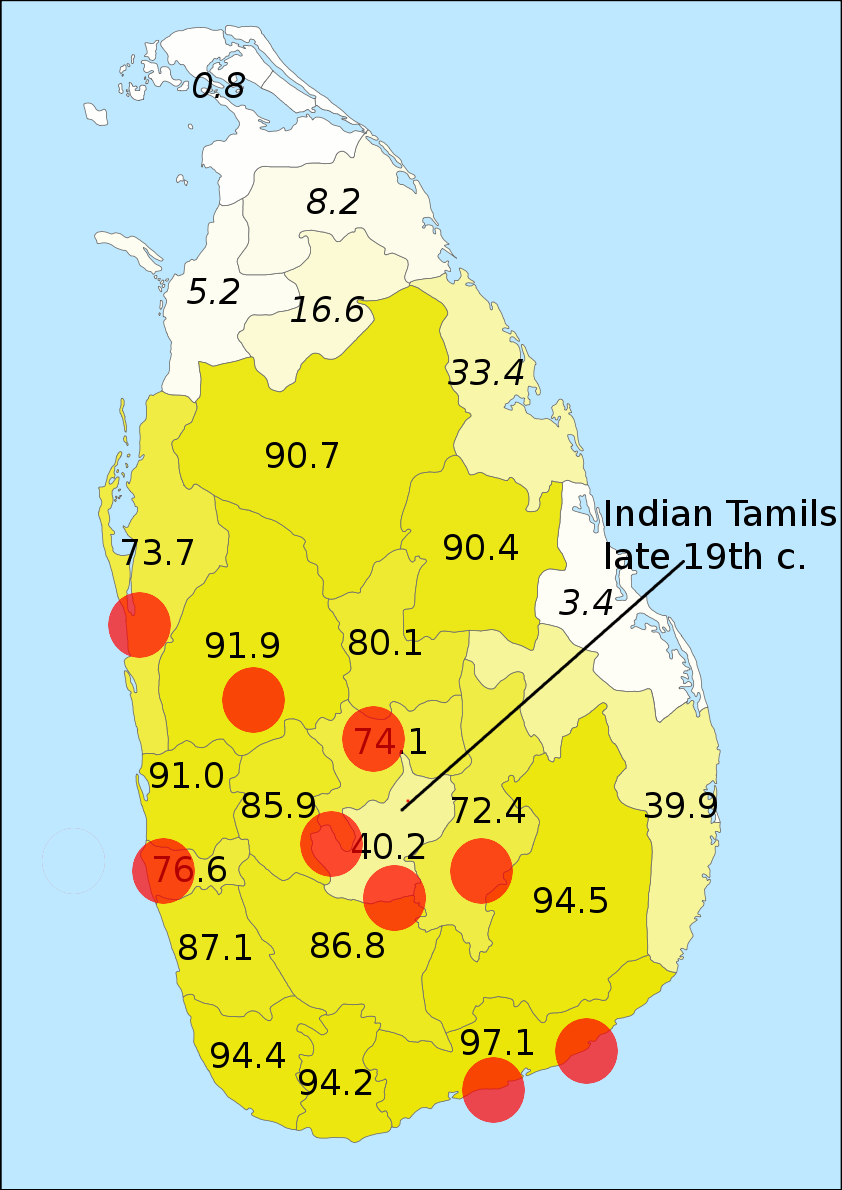
\includegraphics[width=.45\textwidth]{SriLankaSinhalese} 
}
\subfigure[Distribution of the Moor population]{
 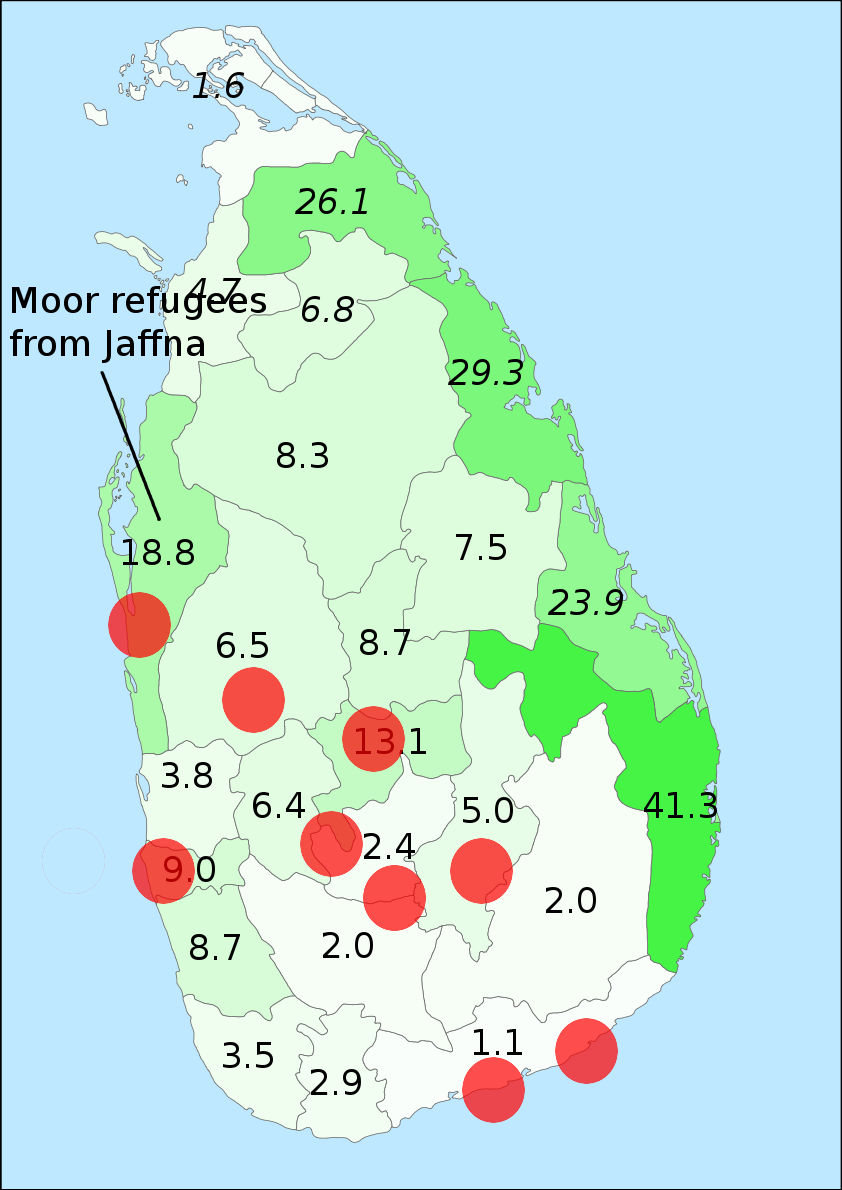
\includegraphics[width=.45\textwidth]{SriLankaMoor} 
 }
 \caption{Demographics of Sri Lanka. Dots mark main towns with Malay population. The Malay population centers are all in the Sinhala speaking area. Recent shifts in population leading to a skewed picture with regard to the early 19th century are indicated.}
\label{fig:maps}
\end{sidewaysfigure}


In the linguistic ecology of 19th century Sri Lanka, Sinhala (and different forms of Tamil) played the role of language of wider communication. Malay (and other minority languages like Sri Lanka Portuguese \citep{Smith1979} or Malayalam \citep{Senaratne2005}) were in-group languages. Settings of this kind have been investigated in other areas of the world and show recurring patterns with regard to the types of language change we find.

One of the earliest cases described in such a setting is Cappadocian Greek \citep{Dawkins1916}. The Greeks having settled down in Cappadocia in the 5th century found themselves surrounded by Turks after the Seljuk invasion in the 11th century, who spoke a language which differed widely from theirs in phonology, morphology and syntax. Being enormously outnumbered, the Greeks had to become fluent in this language of wider communication. This fluency in two languages did not fail to have an impact on their home tongue: Cappadocian Greek has changed its phonology (final devoicing, uvular stops), morphology (agglutinative structure, passive formation, pluperfect formation), syntax (left-branching word order), and semantics (accusative only for definite referents, Turkish idioms), all on the basis of a Turkish model. This lead \citet[198]{Dawkins1916} to the formulation that ``the body has remained Greek, but the soul has become Turkish.'' Crucially, ``[t]here is no indication that Turkish speakers have shifted in any significant number to Greek'' \citep[251f]{ThomasonEtAl1988}. This is identical to Sri Lanka, where there is no reason to assume that any significant number of Sinhalese acquired Malay.\footnote{The
  issue is more complicated for the Moors, but this group was not material in bringing about Sinhala influence.
}
 
% effects of Turkish vowel harmony n/a
% final consonants unvoiced n/a
% Velars kept unaltered in paradigms n/a
% \gamma sounded like qaf n/a
% Failure to pronounce \theta and \delta n/a
% Loss of genders n/a
% partial disuses of the article  (+)
% accusative only used after the article [in definite contexts] (+)
% agglutinative declension +
% comparative of adjectives on Turkish model +
% Use of Turkish numerals -
% Turkish derivative verbal suffixes -
% Personal endings of Turkish added to the Greek verb -
% Imperfect passive fromed agglutivantively +
% pluperfect on Turkish model +
% Positition of enclitic substantive verb
% Borrowing of Turkish idioms +
% Use of turkish word order +
% \citep[203]{Dawkins1916}


The linguistic changes we find in Cappadocian Greek are similar in kind and extent to what we find in Sri Lanka Malay. There is not a complete adaption of the larger language's grammar, but an impressive restructuring of all linguistic subsystems to align more closely with the language of wider communication. The social setting is comparable as well: The Greeks formed a close-knit community differentiated by the surrounding Turks by language, religion, and culture. However, as time progressed, acculturation took place and other parts of culture also became more Turkish, similar to what happened in language. This is also what we find in Sri Lanka, where dress and food of the Malays comply with the Sri Lankan model rather than with the Indonesian one. A difference is that religion is being maintained in Sri Lanka, while some Islamization of Cappadocian Greeks took place \citep[215]{ThomasonEtAl1988}.

The Cappadocian Greek setting is similar to Sri Lanka Malay in another respect: both communities are conscious that they are in the diaspora, and that somewhere out there, there is the metropolis where the homeland of the language lies. The Cappadocian Greek setting is well described and has received some discussion in the literature on language contact since \citet{ThomasonEtAl1988}, but the precise processes leading to the particular structure are not explicated in detail.

This is different in the next language contact situation I want to discuss. On Karkar Island off the north coast of New Guinea, the language of the Takia people  has changed its originally Oceanic grammar to comply with the surrounding Papuan languages, most notably Waskia. This has been described and analyzed extensively by Malcolm Ross under the rubric of metatypy \citep{Ross1996,Ross1997,Ross2001,Ross2007}. Takia adapted word order, semantics of adpositions, and lexical structure of compounds from Waskia. Ross argues that this can only happen when an internally tightly-knit group uses one or more secondary lects/languages to communicate with other groups they are in contact with. Their primary lect/language, however, is the in-group lect/language. \citet[189]{Ross2003diagnosing} offers the following psychological explanation for this, based on principles of economy:

\begin{quote}

[L]exical calquing a[n]d metatypy are driven by a natural tendency to relieve the bilingual speakers' mental burden by expressing meanings in matching ways in both the primary and the secondary lect. The secondary lect wins out because it is the language of the larger community and is slower to change. Grammatical features of the primary lect are allowed to change because it is usually a lects' lexicon (and sometimes also its intonation) that is emblematic of its speakers' identity, not its syntax, so syntax may change without loss of emblematicity. Change begins at the level of the clause because the clause is, roughly, the unit which expresses the speech act, and speakers achieve their first reduction in burden by achieving speech-act equivalence between the two lects. Each set of changes at the next lower syntactic rank represents a further reduction in burden.

\end{quote}

Ross coined the terms `exoteric' for the language of wider communication and `esoteric' for the in-group language. Under metatypy, the esoteric language takes over the grammatical structures of the exoteric language due to cognitive pressure but resists language shift due to the emblematic function of the esoteric language for the group identity of its speakers. 

It seems fair to say that the Malay language in Sri Lanka was an esoteric language. It was confined to Malay speaking homes and annex domain like barracks of the Malay regiment. It was not used as a medium of inter-ethnic communication. This role was reserved for Sinhala (and Tamil, to which I will return below). However, their origin in the Indonesian archipelago was an important part of Malay identity. This can be seen from the fact that even today most Malays trace their ancestry to exiled Javanese princes, a link which is more often than not quite tenuous. The geographical origin of family names is also preserved and a topic of discussion. The in-group language thus served as a marker of identity, which could not be given up \citep[cf.][]{Rassool2010}. However, the grammatical structure was slowly but surely invaded by Lankan structures, which encroached on the language in the same way Turkish encroached on Greek, and Takia, on Waskia.

This type of language change is also attested in South Asia: \citet{Nadkarni1975} describes how the in-group language Karnataka Sarasawat Konkani changed its structure to comply with the structure of the language of wider communication, Kannada. Nadkarni analyzes this as a reduction of cognitive pressure: using the same constructions in both languages lessens the cognitive load speakers have to support.

As far as Malay varieties are concerned, we find a comparable case by the Nonthaburi Malays in Thailand \citep{Tadmor1992,Tadmor1995phd,Tadmor2004}. The Nonthaburi Malays are descendants of war captives from the 18th century or earlier. They live in a Thai-speaking environment, but maintain the Malay language and Islamic faith. The parallels with Sri Lanka are obvious: the time scale is two to three  centuries; the reason for the displacement is warfare; the speakers are isolated and remote from the homeland; they are in a country where their religion is a minority \citep[527]{Tadmor2004}; the differences in size between the in-group languages and the language(s) of wider communication are several orders of magnitude. When we compare the linguistic outcomes, the number of parallels grows even further:

% \begin{quote}
%  The strongest influence is exhibited in grammar and semantics. [...] [Nonthaburi Malay] lost whatever affixation it had inherited from Patani Malay, which was already impoverished compared to Proto-Malay. Productive morphological processes Nonthaburi Malay, such as the use of pseudo-affixes and subjective reduplication, strongly resemble Thai processes. The word order of Nonthaburi has been influence by Thai [...]
%  Thai phonic interference is very significant [...] but not as drastic as the grammatical and semantic interference. [...] Some phonemes were added, although it is not always clear whether this was the result of internal development, interference, or both. [...]
%  Thai interference has been weakest lexically. [...] Since `mixing' with Thai is stigmatized, speakers exert control over lexical borrowing to avoid excessive lexical borrowing from Thai. \citep[317-319]{Tadmor1995phd}
% \end{quote}

\begin{itemize}
 \item Nonthaburi augmented the two Malay stop series by an additional series of aspirated stops under the influence of Thai; SLM added a series of prenasalized stops. Both features are typologically marked.
 \item Nonthaburi developed thriving verb serialization, adopting the semantic and discourse patterns of Thai; Sri Lanka Malay adopted conjunctive participles and clause chains formed with them.
 \item Nonthaburi changed the \em kena\em-passive to align with a Thai model; SLM split the \em kena\em-passive in \em kànà-\em, influenced by Sinhala semantics \citep[407]{Nordhoff2009phd}, and \em kìnna\em, without Sinhala semantics \citep[187ff]{Nordhoff2009phd}.
%  \item There are more changes in syntax in Nonthaburi which resemble to the word order changes in SLM under influence of Sinhala and/or Tamil. Since I reserve the Tamil case for the final section, I do not discuss them further here.
\end{itemize}

\citet[322-323]{Tadmor1995phd} summarizes the linguistic facts as:

\begin{quote}
 Thai interference in Malay is very strong in grammar and semantics, strong in the phonology, and weak in the lexicon. Malay interference in Thai is nonexistent in the grammar and semantics, very weak (if at all) in the phonology, and moderate in the lexicon. In more general terms, Thai interference in Nonthaburi Malay is mostly structural, while Malay interference in Nonthaburi-Malay Thai is mostly lexical. \citep[322-323]{Tadmor1995phd}
\end{quote}

In the context of this paper, we can replace Thai with Sinhala (or Tamil) and Nonthaburi with SLM and the exact same paragraph summarizes the present state of research.

According to Tadmor, the purely linguistic facts point to speakers having shifted from Thai to Malay. However, it is absolutely clear from socio-historical facts that that is not what happened. The direction of shift is rather the reverse one: Malays shift to Thai. The same is true for Sinhalese, who never shifted to Malay.\footnote{As 
 noted above, the case is slightly more complicated for the Moors.
} 
Rather, it is the Malays who become dominant in Sinhala.
Tadmor goes on to argue that it is the language which is primary in every day use (which is not necessarily the maintained language, and not necessarily native) which exerts structural influence.  
\begin{quote}
 Structural interference is usually automatic, and associated with primary $\to$
 secondary language interference, while lexical interference may be controlled, and may therefore be associated with interference in either direction. Unlike what has been claimed in previous studies, it makes no difference if the direction of the interference is from the native (or original, or maintained) language to the second language (or new language, or language shifted to), or vice versa. What matters is which of the two languages, at the time the interference took place, was the primary language of the speaker of the community, and which was the secondary language. \citep[325]{Tadmor1995phd}
\end{quote}

This distinction between primary/wide/exoteric and secondary/narrow/esoteric language can then explain why we find structural patterns from the adstrates in Nonthaburi Malay and Sri Lanka Malay without the slightest sociohistorical evidence of language shift from Thai to Malay, or from Sinhala to Malay. 

It appears that the interplay between languages of wider communication (exoteric) and in-group languages (esoteric), which is found in many other parts of the globe, can account for the Sinhalese influence in Sri Lanka Malay. Given the repeated exposure to certain morphosyntactic constructions and certain phonetic data, and the active production of those by the Malays, these forms became entrenched and eventually made it into the native grammars, where they managed to supplant the traditional forms, very similar to what happened in Cappadocian Greek, Takia, Konkani, or Nonthaburi.

The evidence presented above is difficult to reconcile with the view that Sinhala was not an important contact language. One could of course argue that this is all due to language change after 1956, when nationalist language policies favouring the use of Sinhala were enacted. There are two points which argue against this: The older generation born in the 1930s show the discussed features of Sinhala influence. These structures were already present when they acquired SLM, which was before 1956.

The second point is of phonological nature: the development of phonemic prenasalized stops and phonemic gemination crucially relies on the presence of subphonemic variation in some Malay dialects spoken by the immigrants. Some dialects syllabified clusters of nasal+consonant as .NC, others as N.C . Widely differing grammars are common among immigrant communities, but after some generations, the differences level out \citep{Trudgill1986,Meshtrie1993}. Given that outside of Sri Lanka, no Malay dialect has both N.C and .NC, we expect that Sri Lanka Malay would have chosen one of the two possibilities when the language stabilized,\footnote{The 
 precise date of the stabilization of the language is uncertain, but no later than 1800 is a date commonly assumed.
} 
all other things being equal. But this is not what happened, Sri Lanka Malay has a phonemic distinction. This distinction was clearly facilitated by Sinhala, which also makes this distinction. We thus need dialectal variation in Malay varieties as well as Sinhala influence at the same time. Since dialectal variation in SLM was levelled out by 1800, we have to posit that Sinhala had exerted influence before that date.

The argumentation for geminates is analogous: Voiced geminates are found in Sinhala, but not in Tamil. They occur subphonemically in Malay varieties, but no variety has a phonemic contrast. The most logical explanation for the phonemicization of SLM geminates is adstrate influence, forcing the interdialectal variation to phonemicize. This adstrate influence must have been present before the levelling was completed, i.e. before 1800, and it must have come from Sinhala, since Tamil does not have voiced geminates, unlike Sinhala and SLM.


In this paper, I have surveyed a number of areas where Sinhala contact is sure, or at least very likely. The domains surveyed in this paper suggest that there is actually more influence from Sinhala than from Tamil, but this is due to the topic of this paper being Sinhala influence. Argumentations based on the number of features are of course a difficult enterprise, since it is too easy to stack the deck to come up with any configuration of numbers desirable to defend the thesis. I will therefore not use the data presented in this paper to make any quantitative claims. My claim is rather of a qualitative nature: there has been Sinhala influence in Sri Lanka Malay, and the kind of influence we find suggests that this influence is not a product of the twentieth century alone. This does not conflict with the view that Tamil also had an influence. This is most clearly seen in the lexicon, where Tamil loanwords for basic vocabulary terms like kin or household items are common, but Sinhala loans are all but absent. 

% \subsection{Are Tamil influence and Sinhala influence the result of different processes?}
\section{Conclusion}
In the above section, I have sketched a scenario how Sinhala structures could have entered the Malay language in Sri Lanka. As for Tamil structures, the scenario most often assumed, namely shift from Moorish Tamil to Malay \citep{SmithEtAl2004, SmithEtAl2006cll, Slomanson2006cll}, is different in nature, but led to remarkably similar results. This has led researchers like \citet{Bakker2006, Ansaldo2008genesis} or \citet{Nordhoff2009phd} to suppose that the processes of Tamil influence and Sinhala influence were indeed not that different. If one assumes that Tamil was a language of wider communication with social functions similar to those of Sinhala, the metatypic explanation outlined above becomes available as well \citep{Bakker2006,Ansaldo2008genesis}. More and deeper research into the demographics and social fabric of Ceylonese society of the 19th century will allow to ascertain whether the domains of Tamil use and the domains of the use of Sinhala suggest positing different processes for the respective languages or not. What I hope to have accomplished in this paper is a more modest goal: showing that Sinhala influence was present in Sri Lanka Malay from the early days onwards and outlining the social processes explaining this influence.  This will serve as a base for future investigations of the matter.
  

\bibliographystyle{natuva}
\bibliography{ansaldo,asw,creole,india,phon,malay,sinhala,tamil,nordhoff,lankahist,wortarten,grammars,lgctct,grammaticalization}



\nocite{Verma1976,Gair1998}
\end{document}
